\documentclass[a4paper,11pt,fleqn,twoside,openright,final]{memoir}
%%%%%%%%%%%%%%%%%%%%%%%%%%
%% COMMAND DEACTIVATION %%
%%%%%%%%%%%%%%%%%%%%%%%%%%

\let\added\undefined
\let\deleted\undefined


%%%%%%%%%%%%%%
%% PACKAGES %%
%%%%%%%%%%%%%%


%%% Initial things %%%
% Fix various issues with LaTeX2e
\usepackage{fixltx2e}
% Font package
\usepackage{fourier}
% Index
\usepackage{makeidx}
\makeindex


%%% Translations and character encodings %%%
% Enable use of several characters, including æ, ø and å
\usepackage[utf8]{inputenc}
% Danish language
\usepackage[danish]{babel}
% Use PostScript fonts instead of bitmap ones. Also does other stuff.
\usepackage[T1]{fontenc}
% Various LaTeX symbols
\usepackage{latexsym}
% Wider selection of colours
\usepackage[table]{xcolor}
% Improved element justification
\usepackage{ragged2e}
% Font improvements
\usepackage{fix-cm}
% Enables inclusion of PDF files
\usepackage{pdfpages}
% Enables various forms of lines, like double-underlining (\uuline{})
\usepackage[normalem,normalbf]{ulem}
% Sets the tolerance for distance between words, determining when to hyphenate.
\pretolerance=2500


%%% Figures and tables (Floats) %%%
% Ensures that floats won't appear -before- the place where they're added
\usepackage{flafter}
% Enable multi-rows and -columns
\usepackage{multirow}
\usepackage{multicol}
% Double, horizontal lines
\usepackage{hhline}
% Enables coloured tables
\usepackage{colortbl}
% Gives improved control over placement of floats
% \begin{figure}[!h] % Won't be floating
\usepackage{here}
% Wrap text around figures
\usepackage{wrapfig}
% Wrap text around tables
\usepackage{floatflt}
% Enables the \FloatBarrier command
\usepackage{placeins}
% Rotation of figures
\usepackage{rotating}
% Framed boxes
\usepackage{framed}
% Booktabs - Fancy tables
\usepackage{booktabs}
% Enables inclusion of PDF documents of version 1.6+
\pdfoptionpdfminorversion=6


%%% Mathematic formulas %%%
% AMS math
\usepackage{amsmath}
\usepackage{amssymb}
% Extra fonts (for math, I think)
\usepackage{stmaryrd}
% Access text symbols
\usepackage{textcomp}
% Extend AMS
\usepackage{mathtools}
\usepackage{cancel}
% Use theorems in your document
% The ntheorem package is also used for the example environment
% When using thmmarks, amsmath must be an option as well. Otherwise \eqref doesn't work anymore.
\usepackage[framed,amsmath,thmmarks]{ntheorem}
% Pretty fractions, just because
\usepackage{nicefrac}


%%% Graphics %%%
% Various image-commands
\usepackage{eso-pic}
% Use JPEG and PNG images
\usepackage{array,graphicx}
\DeclareGraphicsExtensions{.pdf,.png,.jpg}
\graphicspath{{./images/}}
%Wrapping Images
\usepackage{wrapfig}


%%% Text stuff %%%
% Filler text
\usepackage{lipsum}
% Page counting
\usepackage{totpages}
% Acronyms
\usepackage{acronym}
%avoid widows
\widowpenalty10000


%%% Source Code Stuff %%%
% Adds \lstinline!code there!, where !! are delimeters not used in the code
% Adds the environment: lstlisting
% Adds command \lstinputlisting[options]{filename.ext}
% More info in manual.
%\usepackage{listings}
%\lstloadlanguages{[Sharp]C,XML,SQL}
%\lstset{numbers=left,
%        numberstyle=\tiny,
%        stepnumber=2,
%        numbersep=5pt,
%        frame=tb,
%        inputencoding=utf8,
%        tabsize=2,
%        extendedchars=true,
%        language=[Sharp]C}

\usepackage{color}
\definecolor{bluekeywords}{rgb}{0.13,0.13,1}
\definecolor{greencomments}{rgb}{0,0.5,0}
\definecolor{redstrings}{rgb}{0.9,0,0}

\usepackage{courier}

\usepackage{listings}

\lstdefinelanguage{JavaScript}{
  keywords={typeof, new, true, false, catch, function, return, null, catch, switch, var, if, in, while, do, else, case, break},
  keywordstyle=\color{blue}\bfseries,
  ndkeywords={class, export, boolean, throw, implements, import, this},
  ndkeywordstyle=\color{darkgray}\bfseries,
  identifierstyle=\color{black},
  sensitive=false,
  comment=[l]{//},
  morecomment=[s]{/*}{*/},
  commentstyle=\color{purple}\ttfamily,
  stringstyle=\color{red}\ttfamily,
  morestring=[b]',
  morestring=[b]"
}


\lstset{language=[Sharp]C,
  captionpos=b,            
  columns=fixed,     
  numbers=left,
  numberstyle=\tiny,
  showspaces=false,
  showtabs=false,
  breaklines=true,
  inputencoding=utf8,
  showstringspaces=false,
  breakatwhitespace=true,
  escapeinside={(*@}{@*)},
  commentstyle=\color{greencomments},
  keywordstyle=\color{bluekeywords},
  stringstyle=\color{redstrings},
  basicstyle=\ttfamily\small,
  literate={ø}{{\o}}1
  		   {æ}{{\ae}}1
  		   {å}{{\aa}}1
  		   {Ø}{{\O}}1
  		   {Æ}{{\AE}}1
  		   {Å}{{\AA}}1
}

\lstdefinestyle{make}{tabsize=4}

%%% References, bibtex and URLs %%%
% Post URLs. Allows breaking at hyphens to help avoid long links.
\usepackage[hyphens]{url}
% Better cross references
\usepackage[danish]{varioref}
% Enable natbib citation styles
\usepackage[numbers]{natbib}
% Define a new 'leo' style for URL package, that will use a smaller font
\makeatletter
\def\url@leostyle{%
  \@ifundefined{selectfont}{\def\UrlFont{\sf}}{\def\UrlFont{\small\ttfamily}}
}
\makeatother
% And of course, use this new style
\urlstyle{leo}




%%% Floats %%%
% Not entirely sure why I need this yet
\let\newfloat\relax
\usepackage{float}
% Enables usage of \subcaption, \subtop and \subbottom
\newsubfloat{figure}


%%% Todo Stuff %%%
% Insert needed corrections with \fixme{..}, which will cause an error during compile, if any are present once 'draft'
% is replaced with 'final'
\usepackage[footnote,draft,danish,silent,nomargin]{fixme}
\fxsetup{layout={footnote,marginclue,index},innerlayout={inline,index}}


%%% Changes Markup %%%
% Markup changes of varying types.
% Adds the commands:
%  - \added[id=(author id), remark={remark text}]{new text}
%  - \deleted[id=(author id), remark={remark text}]{old text}
%  - \replaced[id=(author id), remark={remark text}]{new text}{old text}
\usepackage[xcolor,authormarkup=footnote]{changes}
% Adds the commands:
%  - \cbstart
%  - \cbend
%  - \cbdelete
%  - Environment: changebar
\usepackage[outerbars,xcolor]{changebar}
\cbcolor{red}



%%%%%%%%%%%%%%%%%%%%%%%
%% DOCUMENT SETTINGS %%
%%%%%%%%%%%%%%%%%%%%%%%


%%% Margins %%%
% \setlrmarginsandblock{binding}{edge}{ratio}
\setlrmarginsandblock{3.5cm}{2.5cm}{*}
% \setulmarginsandblock{top}{bottom}{ratio}
\setulmarginsandblock{2.5cm}{3.0cm}{*}
% Performs various calculations and makes several non-Memoir things work with the Memoir class
\checkandfixthelayout 
% Correct todonotes placement
\reversemarginpar


%%% Paragraph formatting %%%
% Size of paragraph indentation
\setlength{\parindent}{0mm}
% Distance between paragraphs (double enter)
\setlength{\parskip}{3mm}
% Line distance
\linespread{1,1}


%%% Bibliography %%%
% Defines parameters for the bibliography, such as the parenthesis and separators
%%%% OLD STYLE!
%\bibpunct{[}{]}{,}{a}{}{;}
% Bibliography style
%%%% OLD STYLE!
%\bibliographystyle{bibtex/harvard}
\bibliographystyle{plainnat}


%%% Table of contents %%%
% Depth of numbered headlines
\setsecnumdepth{subsubsection}
% Changing the document class' limit for number-depth
\maxsecnumdepth{subsection}
% Define the depth included in the table of contents
\settocdepth{section}
% Use letters instead of Roman numerals in TOC
\renewcommand{\thepart}{\Alph{part}}


%%% Text stuff %%%
% Removes distance between items in itemize
%\let\olditemize=\itemize
%\def\itemize{\olditemize\setlength{\itemsep}{-1ex}}
%% Removes distance between items in enumerate
%\let\oldenumerate=\enumerate
%\def\enumerate{\oldenumerate\setlength{\itemsep}{-1ex}}
\usepackage{enumitem}


%%% Changes (Language strings) %%%
\addto\captionsdanish{
  \def\listofchangesname{Ændringer i dokumentet}
  \def\summaryofchangesname{Ændringer}
  \def\changesaddname{Tilføjet}
  \def\changesdeletename{Slettet}
  \def\changesreplacename{Erstattet}
  \def\changesauthorname{Skribent}
  \def\changesanonymousname{anonym}
  \def\changesnoloc{Listen af ændringer tilgængelig efter næste \LaTeX\ kørsel.}
  \def\changesnosoc{Opsummering af ændringer tilgængelig efter næste \LaTeX\ kørsel.}
}


%%% Visual references %%%
% Enables clickable hyperlinks
\usepackage[colorlinks,hidelinks,backref=page]{hyperref}
% General setup of hyperlinks package
\hypersetup{
    breaklinks = true,
    colorlinks = false,
    linkcolor = black,
    anchorcolor = black,
    citecolor = black
}


%%% Colour definitions %%%
% Defines: gray
\definecolor{gray}{gray}{0.80}
% Defines: numbercolor
\definecolor{numbercolor}{gray}{0.7}
% Defines: shadecolor
\definecolor{shadecolor}{RGB}{33,26,82}
% Defines: aaublue
\definecolor{aaublue}{RGB}{33,26,82}


%%% Figure and table texts setup %%%
% Font definition for the 'Figure' or 'Table' displays.
\captionnamefont{\small\bfseries\itshape}
% Font definition for the numbering
\captiontitlefont{\small}
% Delimiter between number and figure text
\captiondelim{. }
% Left justify multi-line figure texts below one another
\hangcaption
% Width of figure text
\captionwidth{\linewidth}
% Distance below figure text
\setlength{\belowcaptionskip}{10pt}
% Fix space between figure number and name
\setlength{\cftfigurenumwidth}{14mm}


%%% Page header and footer %%%
% Define width of header and footer
\setlength{\headwidth}{\textwidth}
% Create pagestyle for pages with and without a new chapter
\makepagestyle{reportPlain}
\makepagestyle{reportChapter}
% Pagestyle for chapter pages (Only a footer, of course)
\makefootrule{reportChapter}{\headwidth}{\normalrulethickness}{\footruleskip}
\makeevenfoot{reportChapter}{\thepage}{}{}
\makeoddfoot{reportChapter}{}{}{\thepage}
% Pagestyle for regular pages
\makerunningwidth{reportPlain}{\headwidth}
\makeheadposition{reportPlain}{flushright}{flushleft}{flushright}{flushleft}
\makeevenhead{reportPlain}{\leftmark}{}{}
\makeoddhead{reportPlain}{}{}{\rightmark}
\makeevenfoot{reportPlain}{\thepage}{}{}
\makeoddfoot{reportPlain}{}{}{\thepage}
\makeheadrule{reportPlain}{\headwidth}{\normalrulethickness}
\makefootrule{reportPlain}{\headwidth}{\normalrulethickness}{\footruleskip}
% Use pagestyles
\pagestyle{reportPlain}
\aliaspagestyle{chapter}{reportChapter}
\aliaspagestyle{part}{reportChapter}
\aliaspagestyle{title}{empty}
% Do not stretch pages
\raggedbottom


%%% Naming %%%
% Define various names for captions and such
\addto\captionsdanish{
  \renewcommand\appendixname{Bilag}
  \renewcommand\contentsname{Indholdsfortegnelse} 
  \renewcommand\appendixpagename{Bilag}
  \renewcommand\cftchaptername{\chaptername~}
  \renewcommand\cftappendixname{\appendixname~}
  \renewcommand\appendixtocname{Bilag}
}


%%% Appendix setup %%%
% Appendix setup. Might need some settings here
\usepackage{appendix}


%%% Chapter look and feel %%%
% Define style: jenor
\newif\ifchapternonum
\makechapterstyle{jenor}{
  \renewcommand\printchaptername{}
  \renewcommand\printchapternum{}
  \renewcommand\printchapternonum{\chapternonumtrue}
  \renewcommand\chaptitlefont{\fontfamily{pbk}\fontseries{db}\fontshape{n}\fontsize{25}{35}\selectfont\raggedleft}
  \renewcommand\chapnumfont{\fontfamily{pbk}\fontseries{m}\fontshape{n}\fontsize{1in}{0in}\selectfont\color{numbercolor}}
  \renewcommand\printchaptertitle[1]{%
    \noindent
    \ifchapternonum
    \begin{tabularx}{\textwidth}{X}
    {\let\\\newline\chaptitlefont ##1\par}
    \end{tabularx}
    \par\vskip-2.5mm\hrule
    \else
    \begin{tabularx}{\textwidth}{Xl}
    {\parbox[b]{\linewidth}{\chaptitlefont ##1}} & \raisebox{-15pt}{\chapnumfont \thechapter}
    \end{tabularx}
    \par\vskip2mm\hrule
    \fi
  }
}
% Use style: jenor
\chapterstyle{jenor}


%%%%%%%%%%%%%%%%%%%%%%%%%%%%%%%%%%%%%%%%%%%%%%%%
% An example environment (http://kom.aau.dk/~jkn/latex/latex.php)
%%%%%%%%%%%%%%%%%%%%%%%%%%%%%%%%%%%%%%%%%%%%%%%%
\theoremheaderfont{\normalfont\bfseries}
\theorembodyfont{\normalfont}
\theoremstyle{break}
\def\theoremframecommand{{\color{aaublue!50}\vrule width 5pt \hspace{5pt}}}
\newshadedtheorem{exa}{Eksempel}[chapter]
\newenvironment{example}[1]{%
		\begin{exa}[#1]
}{%
		\end{exa}
}


%%% Misc stuff %%%
% Use regular numbers for pages
\pagenumbering{arabic}
% Word and letter counts
\newcommand{\wordcount}{\input{preamble/sums/wordcount.sum}}
\newcommand{\charcount}{\input{preamble/sums/charcount.sum}}
\newcommand{\lettercount}{\charcount}
\newif\ifcounts
% Italicized quote-environment
\newenvironment{italicquote}{\begin{quote}\itshape}{\end{quote}}
% Acronyms in list or not (true if in list)
\newif\ifAcroList
\AcroListfalse


%%% Left-aligning bibliography %%%
%\renewcommand*{\bibfont}{\raggedright}


%%%% these patches ensure that the backrefs point to the actual occurrences of the citations in the text, not just the page or section in which they appeared
%%%% http://tex.stackexchange.com/questions/54541/precise-back-reference-target-with-hyperref-and-backref
%%%% BEGIN BACKREF DIRECT PATCH, apply these AFTER loading hyperref package with appropriate backref option
% The following options are provided for the patch, currently with a poor interface!
% * If there are multiple cites on the same (page|section) (depending on backref mode),
%   should we show only the first one or should we show them all?
\newif\ifbackrefshowonlyfirst
\backrefshowonlyfirstfalse
%\backrefshowonlyfirsttrue
%%%% end of options
%
% hyperref is essential for this patch to make any sense, so it is not unreasonable to request it be loaded before applying the patch
\makeatletter
% 1. insert a phantomsection before every cite, so hyperref has something to target
%    * in case natbib is loaded. hyperref provides an appropriate hook so this should be safe, and we don't even need to check if natbib is loaded!
\let\BR@direct@old@hyper@natlinkstart\hyper@natlinkstart
\renewcommand*{\hyper@natlinkstart}{\phantomsection\BR@direct@old@hyper@natlinkstart}% note that the anchor will appear after any brackets at the start of the citation, but that's not really a big issue?
%    * if natbib isn't used, backref lets \@citex to \BR@citex during \AtBeginDocument
%      so just patch \BR@citex
\let\BR@direct@oldBR@citex\BR@citex
\renewcommand*{\BR@citex}{\phantomsection\BR@direct@oldBR@citex}%

% 2. if using page numbers, show the page number but still hyperlink to the phantomsection instead of just the page!
\long\def\hyper@page@BR@direct@ref#1#2#3{\textit{\hyperlink{#3}{Side #1}}}

% check which package option the user loaded (pages (hyperpageref) or sections (hyperref)?)
\ifx\backrefxxx\hyper@page@backref
    % they wanted pages! make sure they get our re-definition
    \let\backrefxxx\hyper@page@BR@direct@ref
    \ifbackrefshowonlyfirst
        %\let\backrefxxxdupe\hyper@page@backref% test only the page number
        \newcommand*{\backrefxxxdupe}[3]{#1}% test only the page number
    \fi
\else
    \ifbackrefshowonlyfirst
        \newcommand*{\backrefxxxdupe}[3]{#2}% test only the section name
    \fi
\fi

% 3. now make sure that even if there is no numbered section, the hyperref's still work instead of going to the start of the document!
\RequirePackage{etoolbox}
\patchcmd{\Hy@backout}{Doc-Start}{\@currentHref}{}{\errmessage{I can't seem to patch backref}}
\makeatother
%%%% END BACKREF PATCHES


% Enable figures like checkmarks
\usepackage{pifont}
\newcommand{\cmark}{\ding{51}}%
\newcommand{\xmark}{\ding{55}}%

%%%%%%%%%%%%%%%%%%%%%%%%%%%%%%%%%%%%%%%%%%%%%%%%
%Flowchart
\usepackage{tikz}
\usetikzlibrary{shapes.geometric, arrows, positioning}
%%%%%%%%%%%%%%%%%%%%%%%%%%%%%%%%%%%%%%%%%%%%%%%%

%\usepackage{bera}% optional: just to have a nice mono-spaced font

\newcommand*\rot{\rotatebox{90}}

\colorlet{punct}{red!60!black}
\definecolor{background}{HTML}{EEEEEE}
\definecolor{delim}{RGB}{20,105,176}
\colorlet{numb}{magenta!60!black}

\lstdefinelanguage{json}{
    basicstyle=\normalfont\ttfamily,
    numbers=left,
    numberstyle=\scriptsize,
    stepnumber=1,
    numbersep=8pt,
    showstringspaces=false,
    breaklines=true,
    frame=lines,
    backgroundcolor=\color{background},
    literate=
     *{:}{{{\color{punct}{:}}}}{1}
      {,}{{{\color{punct}{,}}}}{1}
      {\{}{{{\color{delim}{\{}}}}{1}
      {\}}{{{\color{delim}{\}}}}}{1}
      {[}{{{\color{delim}{[}}}}{1}
      {]}{{{\color{delim}{]}}}}{1},
}
% Preamble additions
%%%% Acronyms %%%

% Add acronyms here, using \acrodef{acronym}[short name]{full name}
%   or \acro{acronym}[short name]{full name}
% Afterwards, these can be referred to as \ac{acronym}

\begin{acronym}
\end{acronym}

%%% Changes (Authors) %%%
\definechangesauthor[name={Mathias Corlin Mikkelsen}, color=orange]{CK}
\definechangesauthor[name={Marc Thorgersen}, color=blue]{MT}
\definechangesauthor[name={Morten Pedersen}, color=brown]{NS}
\definechangesauthor[name={Mathias Sass Michno}, color=olive]{TN}
\definechangesauthor[name={Troels Krøgh}, color=teal]{TK}
\definechangesauthor[name={Søren Frandsen}, color=violet]{SF}

% Define valid hyphenations in cases where TeX falls short
\hyphenation{hvad hvem hvor}

% Comment out the following to remove word and letter counts
\countstrue
% Reference definition
\usepackage[danish]{cleveref}
\crefname{exa}{eksempel}{eksempler}
\newcommand{\myref}[1]{\vref{#1}}
\newcommand{\Myref}[1]{\Vref{#1}}
\begin{document}
\sloppy
% Front matter starts here
\frontmatter
% Insert front page
%\thispagestyle{empty}

%\AddToShipoutPicture*{\put(0,0){
\includegraphics{images/frontpage.pdf}}}

%\hphantom{ }

%  A simple AAU report template.
%  2013-03-06 v. 1.0.0
%  Copyright 2010-2013 by Jesper Kjær Nielsen <jkn@es.aau.dk>
%
%  This is free software: you can redistribute it and/or modify
%  it under the terms of the GNU General Public License as published by
%  the Free Software Foundation, either version 3 of the License, or
%  (at your option) any later version.
%
%  This is distributed in the hope that it will be useful,
%  but WITHOUT ANY WARRANTY; without even the implied warranty of
%  MERCHANTABILITY or FITNESS FOR A PARTICULAR PURPOSE.  See the
%  GNU General Public License for more details.
%
%  You can find the GNU General Public License at <http://www.gnu.org/licenses/>.
%
\thispagestyle{empty}
\pdfbookmark[0]{Front page}{label:frontpage}%
  \addtolength{\hoffset}{0.5\evensidemargin-0.5\oddsidemargin} %set equal margins on the frontpage - remove this line if you want default margins
  \noindent%
  \begin{tabular}{@{}p{\textwidth}@{}}
    \toprule[2pt]
    \midrule
    \vspace{0.2cm}
    \begin{center}
    \Huge{\textbf{
      P3: ProjectFood% insert your title here
    }}
    \end{center}
    \begin{center}
      \Large{
        - Udvikling af applikationer \\fra brugere til data, algoritmer og test\\ og tilbage igen -% insert your subtitle here
      }
    \end{center}
    \vspace{0.2cm}\\
    \midrule
    \toprule[2pt]
  \end{tabular}
  \vspace{2cm}
  \begin{center}
    {\large
      Projektrapport%Insert document type (e.g., Project Report)
    }\\
    \vspace{0.2cm}
    {\Large
      DS304E14%Insert your group name or real names here
    }
		\vspace{2 cm}
		\begin{flushleft}
			\parindent=2 cm
			\Large
      \begin{minipage}{0.45\textwidth}
      \centering
      \rule{\textwidth}{0.5pt}\\
			\textit{Mathias Corlin Mikkelsen}
      \end{minipage}
		\end{flushleft}
		\begin{flushright}
			\hangindent=2 cm
			\Large
      \begin{minipage}{0.45\textwidth}
      \centering
      \rule{\textwidth}{0.5pt}\\
			\textit{Marc Tom Thorgersen}
		  \end{minipage}
    \end{flushright}
		\begin{flushleft}
			\parindent=2 cm
			\Large
      \begin{minipage}{0.45\textwidth}
      \centering
      \rule{\textwidth}{0.5pt}\\
			\textit{Morten Pedersen}
		  \end{minipage}
    \end{flushleft}
		\begin{flushright}
			\hangindent=2 cm
			\Large
      \begin{minipage}{0.45\textwidth}
      \centering
      \rule{\textwidth}{0.5pt}\\
			\textit{Mathias Sass Michno}
		  \end{minipage}
    \end{flushright}
		\begin{flushleft}
			\hangindent=2 cm
			\Large
      \begin{minipage}{0.45\textwidth}
      \centering
      \rule{\textwidth}{0.5pt}\\
			\textit{Søren Hvidberg Frandsen}
		  \end{minipage}
    \end{flushleft}
		\begin{flushright}
			\hangindent=2 cm
			\Large
      \begin{minipage}{0.45\textwidth}
      \centering
      \rule{\textwidth}{0.5pt}\\
			\textit{Troels Beck Krøgh}
		  \end{minipage}
    \end{flushright}

  \end{center}
  \vfill
  \begin{center}
  Aalborg Universitet\\
  Institut for datalogi\\
  Selma Lagerlöfs Vej 300\\
  9220 Aalborg Ø
  \end{center}
%\clearpage

% Ensure that next page opens on the right
\cleardoublepage
% Insert title page
\thispagestyle{empty}
\enlargethispage*{\ifcounts 4\else 2\fi\baselineskip}
{\samepage
\begin{tabular}{cc}
  \parbox{0.5\textwidth}{ %
    \hspace*{1cm} %
    
\includegraphics[width=4cm,height=4cm,keepaspectratio]{images/aau_logo_da.pdf}} &
  \parbox{0.5\textwidth}{\begin{tabular}{l}
      {\small \textbf{3. Semester --- Software}}\\
      {\small Selma Lagerlöfs Vej 300} \\
      {\small 9210 Aalborg SØ} \\
      {\small http://www.cs.aau.dk/}
    \end{tabular}}
\end{tabular}

\begin{tabular}{cc}
  \parbox{8cm}{
  \begin{description}
    \item { \textbf{Titel:}}\\ 
      ProjectFood
    \item { \textbf{Tema:}}\\ 
      Programering og modelløsning. 
  \end{description}
  
  \parbox{8cm}{
  \begin{description}
    \item { \textbf{Projektperiode:}}\\
      P3 (Efterårssemestret 2014) \newline 02-09-2014 - 19-12-2014
    \hspace{4cm}
    \item { \textbf{Projektgruppe:}}\\
        DS304E14
    \hspace{4cm}
    \item {\textbf{Gruppemedlemmer:}}\\
      Marc Tom Thorgersen\\
      Søren Hvidberg Frandsen\\
      Troels Beck Krøgh\\
      Mathias Corlin Mikkelsen\\
      Morten Pedersen\\
      Mathias Sass Michno\\
    \hspace{2cm}
    \item { \textbf{Vejleder:}}\\
      Thomas Bøgholm\\
    \end{description}
  }

  \begin{description}
    \item { \textbf{Oplagstal:} x}
    \item { \textbf{Rapport sideantal:} x} 
    \item { \textbf{Appendiks sideantal:} x}
    \item { \textbf{Total sideantal:} \ref{TotPages}}
    \item { \textbf{Projekt klaret den:}\\ 19-12-2014} 
    \ifcounts
      \item { \textbf{Ord/Tegn (Cirka):} ...}
    \fi
  \end{description}
  \vfill } &
  \parbox{7cm}{
   \vspace{.15cm}
    \hfill 
    \begin{tabular}{l}
      { Abstract:}\bigskip \\
      \fbox{
      \parbox{6.5cm}{\bigskip
        {\vfill{\small % Abstract indeholder beskrivelse af opgaven, formål/problemstilling, anvendte metoder, resultater
% og konklusioner.

The following project studies how to fuk
        \bigskip}}
      }}
    \end{tabular}}
\end{tabular}
}%samepage end
\\
\vfill
\noindent{\footnotesize{\textit{Rapportens indhold er frit tilgængeligt, men offentliggørelse (med kildeangivelse) må kun ske efter aftale med forfatterne.}}}
% Ensure that next page opens on the right
\cleardoublepage
\chapter{Forord}
Her vil komme tekst om læsevejledning.

Teksten vil beskrive kildehenvisninger, samt kodeeksempler.

Ord som 'vi' referer til forfatterne af rapporten.

 Eventuel beskrivelse af struktur på: CD, bilag og andet.

\cleardoublepage
% Insert table of contents
\thispagestyle{empty}
\tableofcontents*
\label{table_of_contents}
%%%%%%%%%%%%%%
%% CHAPTERS %%
%%%%%%%%%%%%%%
% Main matter starts here
\mainmatter
\part{Analyse}
\chapter{Indledning}\label{chapter:indledning}

I dagligdagen kan det være svært at koordinere indkøb, opskrifter og tilbud således, at dette foregår på en optimal måde. Nogle kigger i tilbudsaviser og planlægger deres indkøb i en eller flere butikker, andre vælger kun at handle i en butik. Hvis ikke man planlægger disse indkøbsture, kan det lede til madspild pga. overindkøb/impulskøb eller for mange unødige ture i supermarkederne, hvilket kan tage tid i ens hverdag. Derudover kan det være problematisk at koordinere, hvem der handler hvad ind med eventuelle samboende.

Det kan også være svært at leve sundt og varieret som fødevareministeriet anbefaler; det kan være svært at finde på noget at lave til aftensmad; eller også har man ikke nogen gode opskrifter, man synes om.
Hvis man planlægger sine indkøb efter opskrifter, skal man holde styr på, hvilke varer man har i sit hjem for at undgå at købe for meget ind. Det kan samtidig være svært at overskue, hvilken butik der er den bedste at handle ind i på et givent tidspunkt, eftersom at tilbud hele tiden ændrer sig og faste priser er forskellige. Det er heller ikke sikkert, at den valgte opskrift man køber ind efter, indeholder varer, som er på tilbud, når man gerne vil have dem - på denne måde ender man måske med at leve dyrere end nødvendigt.

Dette projekt vil undersøge, om man kan gøre det nemmere at handle efter tilbuddene i dagligvarebutikkerne, alt imens man reducerer problemerne vedr. det at beslutte sig for, hvad man skal lave til aftensmad.
Derfor vil der i de følgende afsnit blive udforsket hvad der er på markedet til hjælp med denne problemstilling. Desuden vil der også undersøges personers vaner, samt holdninger til elektronisk hjælp til problemstillingen i form af korte interviews.

\chapter{Metode}\label{chapter:Metode}

Dette kapitel vil gennemgå og evaluere på de metoder som benyttes i forbindelse med projektet.
Slutteligt vil der være en kort beskrivelse af metodernes sammenhæng, samt hvordan de benyttes i gruppen.

\section{Scrum}

Scrum er en process som bruges i forbindelse med udarbejdelse af komplekse problemer som løbende kan udvikle sig. 
Scrum er en simpel process, men kan være svær at udføre godt.
Det bruges ofte i virksomheder hvor man har kunder som kan beskrive hvilke krav der er til projektet, og på denne måde styre \textbf{product backlog}.
Dette er en liste over opgaver der skal løses, og disse skrives ofte som en user story på formen:\\ \\ \textit{''Som en <rolle> vil jeg kunne <mål>''. }\\ \\
Disse user stories vil derefter vælges til et såkaldt sprint som varer 30 dage. 
I disse 30 dage arbejdes der i grupper af normalt 7 for at få alle user stories der er valgt i sprintet til at blive færdige og testet.
Der kan laves et scrumboard for at holde styr på hvilke opgaver der skal laves til hver enkelt user story. 
På denne måde skaber man overblik over opgaverne, og man kan hele tiden se hvad der mangler at blive lavet.
Hver dag når man mødes laver men at Daily Scrum, som er et kort møde, hvorpå man fortæller de andre i gruppen hvad man har lavet, hvad man vil lave i dag, samt problemer man med arbejdet.
En Scrum master sørger for at gruppen følger Scrum, og at Daily Scrum forbliver på sporet. 
Personen står også for alt kontakt mellem gruppen og administrationen ved virksomheden.
Efter et sprint mødes man og evaluerer og fremviser for kunderne hvad man har lavet ved et Sprint review meeting.
På denne måde kan man sørge for at næste sprint bliver bedre end det forrige. 
Men hvordan forholder Scrum sig i forhold til projektet?

\begin{sidewaystable}
    \colorlet{shadecolor}{gray!40}
    \rowcolors{1}{white}{shadecolor}
      \begin{tabular}{p{5cm}p{5cm}p{5cm}p{5cm}}
      %\hline
	       				 & Scrum  & Vores Projekt & Kommentarer  \\ \hline
	   Iterationslængde  		
	   		& 30 dage 
	   		& Der er ikke meget tid til udvikling cirka 2 måneder. 
	   		& Hvis der skulle bruges 30 dages iterationer ville der måske kun kunne laves 2 iterationer\\
	   		
	   Team størrelse    		
	   		& 7 personer
	   		& 6 personer 
	   		& Dette passer fint og kan fungere fint. \\
	   		
	   Kunde involvering 		
	   		& Meget kunde involvering, bl.a. til at styre product backlog.
	   		& Vi har ikke en kunde, men der er potentielle brugere som kan interviewes for at finde frem til deres krav til et produkt.
	   		& Vi kan selv finde kravene og danne user stories, men skal derfor også selv styre product backlog.\\
	   		
	   Kommunikationsmetoder	
	   		& Daily Scrum, Sprint review meeting, Scrum master, kontakt med kunder og administration fra virksomheden.
	   		& Gruppen har et grupperum på universitet, og skal ikke tale med administration. 
	   		& Scrum master rollen kan gå på runde fra sprint til sprint eller fra uge til uge. \\
    \end{tabular}
  \caption{Sammenligningstabel over Scrum og vores projekt.}\label{tabel:sammenligningstabel}
\end{sidewaystable}

Der skal laves ændringer på den traditionelle Scrum process  for at tilpasse det til projektet, men disse kan håndteres og ændres, som \myref{tabel:sammenligningstabel} også viser.

\section{Objekt Orienteret Analyse \& Design}

OOA\&D er en analysemtode som har til formål at finde krav til et system, fastlægge design, og at danne en forståelse for et system, dets omgivelser og hvilke krav der skal til for at implementere det.
Metoden stammer fra bogen af samme navn.\citep{OOA&D2001}
Den gør brug af UML til at beskrive struktur og klasser indenfor området.
Herudover finder metoden:

\begin{itemize}
\item Systemdefinition
\item Hændelser
\item Adfærd for klasserne
\item Funktioner
\item Tilstande i systemet
\item Aktører og deres brugsmønstre til systemet.
\end{itemize}

Med alle disse elementer kan laves et analyse- og designdokument.
Med disse dokumenter kan man nemmere lave et godt og velovervejet design.
Dog har vi valgt ikke at finde adfærd for klasserne, da dette var set som værende overflødigt.
Det beskriver klasserne, hvornår de laves i systemet, og gennemgangen af alle klassernes hændelser. 
Dokumentationen for disse fylder utroligt meget og selve adfærden er et mellemtrin i metoden, til at danne en god struktur, derfor dokumenteres strukturen i stedet.
De andre analyse dele er meget centrale og hjælper med at beskrive systemet og er derfor taget med. 

Scrum og OOA\&D hjælper projektet på hver sin måde.
Scrum som projektstyring og for at overskueliggøre projektets opgaver. 
En user story ved navn "Rapport" laves, og ud fra denne dannes der opgaver som skal laves i hvert sprint. 
Dette sørger for at rapporten ikke falder bagud i forhold til systemet udvikling.
OOA\&D hjælper derimod med at organisere og strukturere analysen som beskrevet i dette afsnit, og derfor komplimentere de to metoder hinanden udemærket.
Dog fordi Scrum benytter user stories, vil den endelige kravspecifikation ikke være beskrevet på traditionel OOA\&D vis, men i stedet vha. user stories.










\chapter{Problemanalyse}\label{chapter:problemanalyse}
I dette kapitel lægges rammerne for problemet fast.
Problemet er groft defineret, som problematikker i forhold til madlavning og indkøb i hverdagen.

Først foretages nogle indledende interviews der har til formål at bekræfte og klarlægge problemet, samt at undersøge om der er interesse for løsninger til problemet.
Efter dette foretaes en state of the art-analyse der har til formål at undersøge og udforske eksisterende løsninger til problemet.
Der skal altså undersøges hvilke funktionaliteter løsningerne har, samt om løsningerne er tilfredsstillende.
Efter denne undersøgelse, udføres endnu et interview.
Dette interview skal undersøge hvilke funktionaliteter potentielle brugere har interesse for, hvilket gøres i forbindelse med gruppens egen prototype.
Sidst i kapitlet defineres problemformuleringen, som danner grundlag for den resterende del af projektet.

\section{Indledende interview}
Onsdag d. 17 september gennemførte vi en række semi-strukturerede interviews i Aalborg midtby blandt folk omkring Føtex.
Vi adspurgte syv personer i forskellige målgrupper, herunder unge der bor alene, unge der bor sammen med nogen, og  folk over 30 med begge førnævnte sociale statusser.
Aldersspændet var fra 20 - 51, og kønnene var ligeligt fordelt.
Formålet med disse interviews var at danne et basalt overblik over vores problemområde, samt undersøge, hvordan folk håndterede vores initierende problem på nuværende tidspunkt.
Vores interviews bestod af en håndfuld forberedte spørgsmål, samt løsere samtale, for at følge op på disse spørgsmål.
Ud af interviewene fandt vi følgende hovedpunkter:
\begin{itemize}
	\item Generelt er folk uorganiserede når det kommer til indkøb, og især unge mennesker bruger sjældent indkøbslister.
	\item Inspiration til aftensmåltider findes ofte i indkøbssituationen eller ud fra princippet “hvad man lige har lyst til”.
	\item Det er ikke mange, der gennemgår tilbudsaviser, og endnu færre går bevidst efter tilbud.
	Dog kan det påvirke beslutninger om aftensmåltid, hvis en given varer er på tilbud i butikken, hvor der handles ind.
	\item Især den yngre målgruppe (18-28) er interesseret i en løsning med tilbud, indkøbslister og opskrifter til inspiration kædet sammen. Mens den ældre målgruppe (28+) virker mere interesseret i at kunne dele indkøbslister med familie, for bedre at kunne organisere indkøb.
	\item Opskrifter er som sagt noget, der mest interesserer det yngre segment.
	Dog påpeger nogle, at stor tendens til at være kræsen kræver at man kan sætte præferencer.
\end{itemize}

Dog skal det nævnes, at der bør evalueres over designet og funktionaliteterne med brugerne for at sikre et brugbart produkt til slut.
Fremadrettet vil der arbejdes videre med følgende områder:

\begin{itemize}
	\item Indkøbslister
	\item Tilbud
	\item Opskrifter.
\end{itemize}

\section{State of the art}\label{s:SOTA}
I dette afsnit har vi forsøgt at finde en bred vifte af forskellige løsninger der kan løse et eller flere problemer i forbindelse med indkøb og madlavning, omhandlende indkøbslister, tilbud og opskrifter.

Der vil blive kigget på web services og applikationer, der har til formål at løse nogle af de samme problemer, der berører vores emne.
Løsningerne, der er præsenteret i dette afsnit, forsøger at afhjælpe de problemer beskrevet af de adspurgte i interviewene i \myref{section:interview1}.

\subsection{eTilbudsavis}
eTilbudsavis er en online service, der kan findes på deres hjemmeside\footnote{\underline{www.etilbudsavis.dk}}. eTilbudsavis er en online avis med en høj funktionalitet og en nem brugergrænseflade.
Der kan på siden oprettes et login, således der kan findes tilbage til ændringer på et senere tidspunkt eller andre enheder.
eTilbudsavis har tre mærkbare funktioner, som brugeren har adgang til, hvilket er tilbudsaviser, ønske- og indkøbslister og tilbud.

Tilbudsavis-funktionen, hvilket kan ses på \myref{ss:eTilbudsavis}, indeholder også den mulighed at sætte en præference på, hvor stor en radius man vil lede i efter butikkers tilbudsaviser.
Under hver avis, som det ses på figuren, er der også angivet afstand i meter fra ens aktuelle placering.
Der kan vælges imellem alle aviser, som er tilgængelige online og inden for den valgte radius.
Aviserne bliver opdateret løbende, så når der er en ny tilgængelig, bliver den gamle fjernet.
Inde i aviserne kan man trykke på en tilbud, og denne tilføjes til en liste.

\begin{wrapfigure}{o}{0.68\textwidth}
\vspace{-20pt}
	\begin{center}
		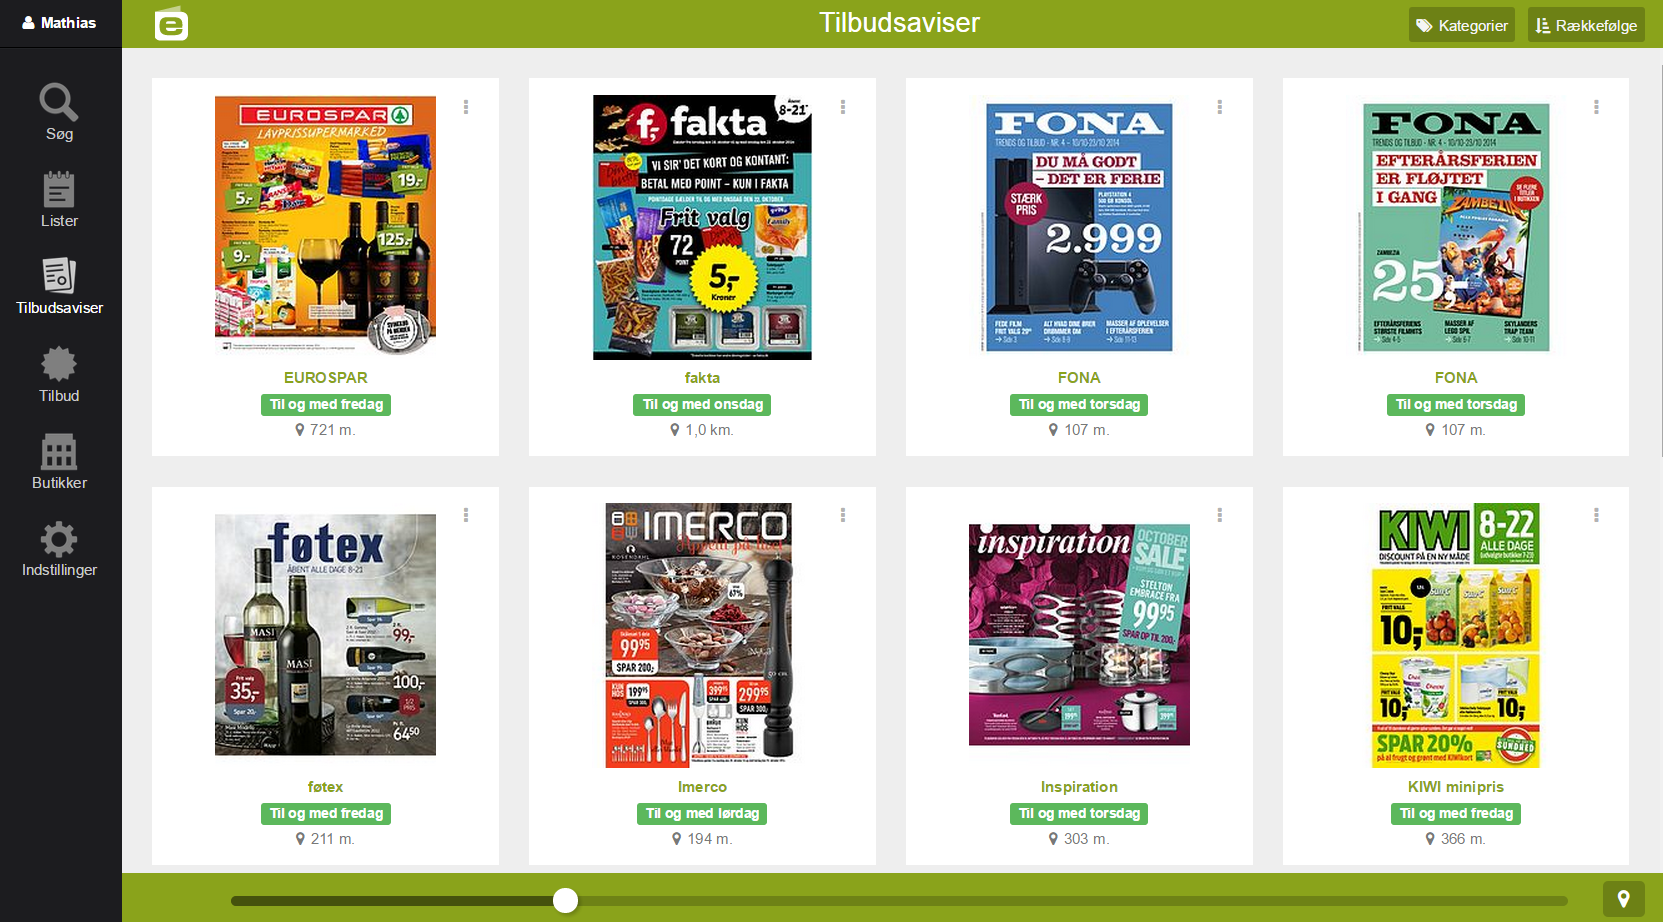
\includegraphics[width=0.66\textwidth]{images/Images/eTilbudsavis.PNG}
	\end{center}
	\vspace{-20pt}
	\caption{Tilbudsaviser på eTilbudsavis.dk}\label{ss:eTilbudsavis}
	\vspace{-20pt}
\end{wrapfigure}

Der er mulighed for at tilføje varer til to lister, en indkøbsliste og en ønskeliste.
Når en vare er valgt, bliver den tilføjet til den valgte liste.
Listen indeholder navn, butik, pris og den valgte mængde, for varen.
Der kan foruden det at vælge varer fra tilbudsaviserne, nemt skrives generiske varer på listen. Varen på listen kan da krydses af for at kunne holde styr på, hvad der er blevet købt.

Hvis der ikke ønskes at skulle bladres tilbudsaviser igennem, er der den mulighed at få vist en hel side kun med tilbud.
Alle aktuelle tilbud fra aviserne, er da vist som elementer med navn, beskrivelse, pris, butik og afstand. Disse tilbud kan på samme måde nemt tilføjes til listerne.

eTilbudsavis er en god online løsning, som har mange gode features, derfor har vi også brugt dem som kilde til vores tilbud gennem deres API.
Dette API er beskrevet i \myref{api}. \myref{Skal vi nævne det allerede her ?}

\subsection{Tilbudsugen}
Tilbudsugen minder på mange måder om eTilbudsavis, og kan findes på deres hjemmeside\footnote{\underline{www.tilbudsugen.dk}}.
Den har samtlige dagligvareaviser, samt flere inden for bl.a. byggemarkeder, og autoudstyr.
De giver et nemt overblik over diverse aviser, og man kan hurtigt og nemt læse dem på nettet.
Der er desuden mulighed for at lave præferencer som ved eTilbudsavis, her kan man bl.a. vælge økologi eller nøglehulsmærket.
Når man tilføjer en vare til indkøbslisten, søger den automatisk efter tilbud på den valgte vare.
Man bliver bedt om at vælge et specifikt tilbud, og netop dette tilbud bliver tilføjet til indkøbslisten med pris, butik, udløbsdato, mængde og et billede af varen.
Man kan som i eTilbudsavis også trykke på en vare direkte i avisen for at tilføje den til sin liste.
Hvis man vil dele sin indkøbsliste, er det også en mulighed vha. en ``delekode'' som man kan give til en anden bruger - de kan på denne måde også se listen.
Funktionerne findes på hjemmesiden, men det er ikke altid de virker.
For eksempel hvis man tilføjer noget uden at angive et antal, og du så prøver at dele listen med en, vil de ikke være at finde på listen.
Desuden kan man ikke ændre på antallet af varen, du allerede har sat på din indkøbsliste.
For at opnå dette, skal man slette varen, og tilføje den igen med det nye antal.
De har desuden også en smartphone app, men denne crasher ofte, når man benytter sig af deres indkøbsliste, men fungerer tilgengæld fint, hvis man blot vil se på ugens tilbud i aviserne.

Tilbudsugen er et lidt dårligere alternativt til eTilbudsavis, da der er problemer med delbarheden af indkøbslisterne, samt den app, der er stillet til rådighed, ikke er stabil.
Derimod er den nem at navigere, siden er brugervenlig og ser overskuelig ud.

\subsection{Smartphone Apps udgivet af butikker}
På \myref{tbl-smartphone} ses der nogle butikskæder, som har udviklet android apps, samt hvilke funktionaliteter disse har.
For at skabe et overblik, er der udvalgt features, og disse er blevet opsat i et skema for overskuelighedens skyld.
\begin{table}[H]
	\centering
		\colorlet{shadecolor}{gray!40}
    	\rowcolors{1}{white}{shadecolor}
	    \begin{tabular}{l|lllllllllll}
	    %Table: http://bit.ly/1tD6EI6
	   	%Funktionalitet & Tilbudsavis & Indkøbsliste & Opskrifter & Varescan & Find butik & Budget & Madplan & Rabatkupon/fordelsordning & Deling af indkøbslister & Rating på Play & Senest opdateret \\ \hline
	     & \rot{Tilbudsavis} & \rot{Indkøbsliste} & \rot{Opskrifter} & \rot{Varescan} & \rot{Find butik } & \rot{Budget} & \rot{Madplan} & \rot{Rabatkupon} & \rot{Deling} & \rot{Play rating} & \rot{Senest} \rot{opdateret} \\ \hline
	   	Føtex                       & \cmark   & \cmark    & \cmark  & \cmark   & \cmark  & ~      & ~       & ~          & ~                       & 3.4 (354)      & 2014-07-24       \\
	    SPAR                        & \cmark   & \cmark    & \cmark  & ~        & \cmark  & \cmark & ~       & ~          & ~                       & 2.8 (64)       & 2014-05-15       \\
	    Fakta                       & \cmark   & \cmark    & \cmark  & ~        & \cmark  & ~      & \cmark        & \cmark     & \cmark               & 3.1 (454)      & 2014-08-02       \\
	    FaktaQ                      & \cmark   & ~         & \cmark  & ~        & \cmark  & ~      & ~       & ~          & ~                       & 4.4 (7)        & 2014-03-11       \\
	    REMA 1000                   & \cmark   & \cmark    & \cmark  & ~        & \cmark  & ~      & ~       & ~          & ~                       & 3.5 (674)      & 2014-04-16       \\
	    SuperBrugsen                & \cmark   & \cmark    & \cmark  & ~        & \cmark  & ~      & ~       & ~          & ~                       & 3.8 (987)      & 2014-06-30       \\
	    Kvickly                     & \cmark   & \cmark    & \cmark  & ~        & \cmark  & ~      & ~       & ~          & ~                       & 3.7 (632)      & 2014-07-20       \\
	    \end{tabular}
	    \caption{Nogle butikskæder med smartphone apps samt deres funktionaliteter.}\label{tbl-smartphone}
	\end{table}
Vi har valgt at beskrive en af disse apps nærmere, og valget faldt på Faktas app, MitFakta, da denne bliver opdateret og har flest funktioner.
\subsubsection{Faktas Android App}

\begin{wrapfigure}{o}{0.4\textwidth}
\vspace{-20pt}
	\begin{center}
		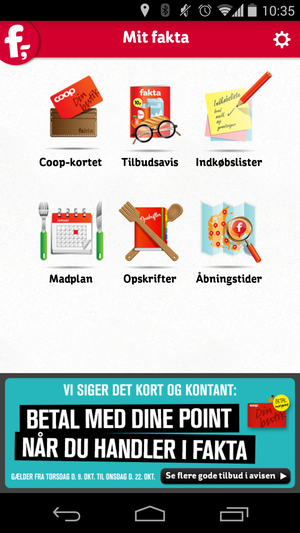
\includegraphics[width=0.38\textwidth]{images/Images/MitFakta.png}
	\end{center}
	\vspace{-20pt}
	\caption{MitFakta}
	\vspace{-20pt}
	\label{ss:MitFakta}
\end{wrapfigure}

Faktas android app er som helhed overskuelig.
Efter åbning af appen kan man vælge mellem seks menupunkter eller ændre sine indstillinger, disse kan ses på \myref{ss:MitFakta}.
Første menupunkt omhandler ``Coop-kortet'', og giver brugeren mulighed for at indtaste sine medlemsinfomationer, da disse giver særlige tilbud.
Andet menupunkt er deres tilbudsavis, hvilket er en digital kopi af den fysiske tilbudsavis.
Dog kan man fra den også tilføje varer til sin indkøbsliste, eller se varerne i et gitterformat.
Tredje menupunkt er ``indkøbsliste'', her kan man have flere personlige og/eller delte indkøbslister.
Her kommer deres Facebook integration også i spil, som tillader nem deling af indkøbslister med brugerens Facebook venner.
Fjerde menupunkt er en madplan, hvori man kan planlægge sin egen madplan, eller se Faktas anbefalinger til en ``under 20 kr pr. person pr. aften''-løsning.
Femte menupunkt er deres opskrifter.
Her findes der et stort antal af opskrifter, disse kan tilføjes direkte til ens madplan eller indkøbslister (både personlige og delte).
Sjette menupunkt hedder ``Åbningstider'', og her kan brugeren finde Faktas butikker samt deres forskellige åbningstider.

Appen virker rigtig godt, der er ingen blindgyder, og derfor er den meget nem at navigere rundt i. Der er lagt megetxnote{Meget alligevel?} fokus på den sociale del, da der kan deles med venner på facebook, hvilket simplificerer delingen af indkøbslister. Den eneste ulempe, der er ved denne app, er, at den kun er egnet til vare fra Fakta, og derfor sætter en del restriktioner på sig selv.

\subsection{Tøm køleskabet} \fxnote{Er dette afsnit relevant længere, vi bruger det jo ikke senere? - Troels Jeg tænker vi kan prøve at bruge det senere, vi afgrænser os vel fra at lave lagerstyrring eller tøm køleskabet, det var nok tanken at det var det vi ville da dette blev skrevet? - Søren}
Der findes talrige tjenester, der tilbyder ``at tømme dit køleskab''.
Mere specifikt, tilbyder de en service, hvor du som bruger, angiver hvilke varer dit køleskab pt. indeholder, samt hvilke andre ingredienser du har til rådighed.
Derefter får du så præsenteret en række forskellige opskrifter, der kan laves ud fra dine tilgængelige ingredienser.
De fleste af tjenesterne (herunder dem vi her har undersøgt) viser også opskrifter, som indeholder yderligere ingredienser.
Dette betyder naturligvis, at man som bruger ikke bliver fritaget fra at handle ind, hvis man mangler nogle ingredienser til lige netop den opskrift, man vælger at udføre.
Tjenesten \textit{MyFridgeFood} \footnote{\underline{www.myfridgefood.com}} tilbyder at oprette en indkøbsliste ud fra netop disse manglende ingredienser, hvilket kan lade sig gøre blandt andet fordi, alle opskrifter er interne på \textit{MyFridgeFood}.
I modsætning til dette er der \textit{Supercook} \footnote{\underline{www.supercook.com}}, som linker til eksterne opskrifter, og ikke tilbyder at generere en indkøbsliste.
Umiddelbart anbefales opskrifter ikke ud fra den enkelte brugers smag og madvaner, men udelukkende på baggrund af, hvad man ``har i køleskabet''.
Grundet dette virker tjenesterne mere som simple filtreringer af databaseopslag, end egentlige anbefalinger, der tager højde for brugerens smag og præferencer indenfor den gastronomiske verden.

Som vi har set i ovenstående gennemgang, findes der alternativer til den klassiske indkøbstur, der er dog ingen af disse, der formår at løse alle problemerne.
Ved alle løsningerne opstår også nye ulemper og problemstillinger i forhold til almindeligt indkøb.
Alt taget i betragtning vil det komme meget an på nuværende vaner og familiestrukturen, om disse muligheder vil være en god løsning for en given familie.

\section{Prototype interviews}\label{section:interview2}
State of The Art undersøgelsen viste at der er mange forskellige løsninger, men der er også mange mangler i disse alligevel.
Ingen af løsningerne tager tilbud fra alle butikker, har indkøbsliste, tilbyder opskrifter der er integreret med tilbudene, samt vurdering af disse.
Løsningerne
Derfor har vi udformet en prototype i Microsoft Office Powerpoint som viser forskellige funktionaliteter.
Diasshowet består af forskellige skærmbilleder, som der kan navigeres imellem ved tryk på de gule felter.

Et eksempel kan ses på \myref{ss:Prototype}.

\begin{wrapfigure}{o}{0.68\textwidth}
\vspace{-20pt}
	\begin{center}
		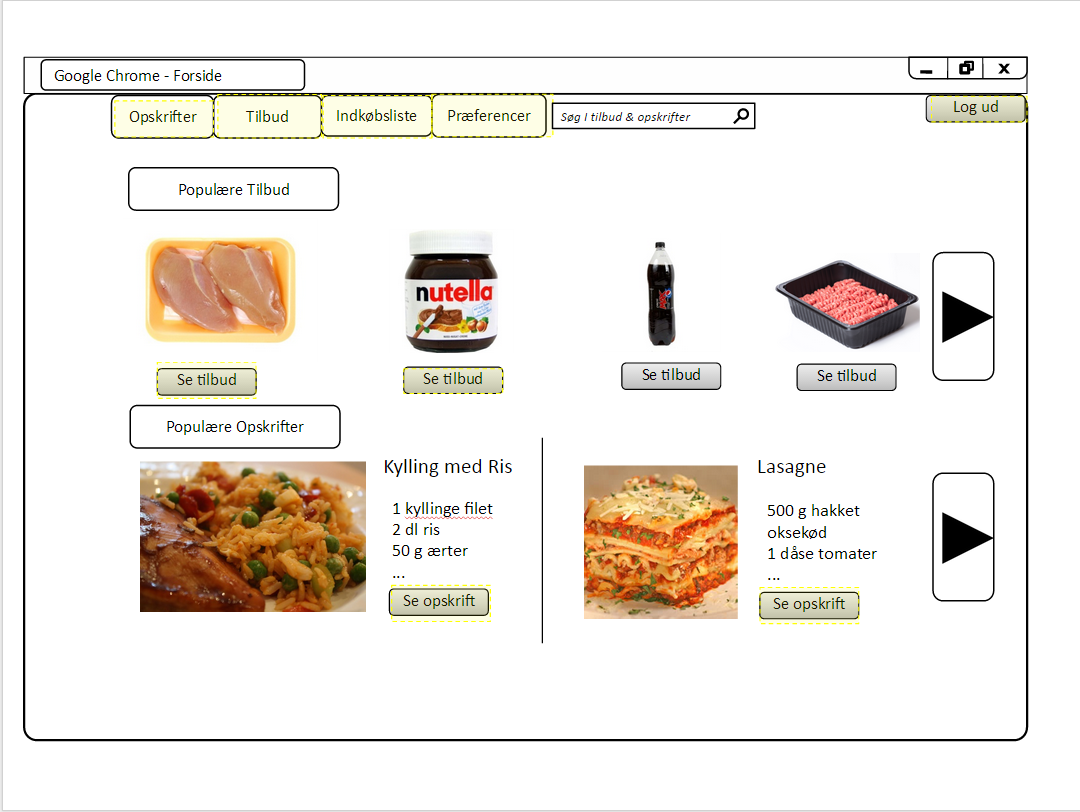
\includegraphics[width=0.66\textwidth]{images/Images/prototype-forside.PNG}
	\end{center}
	\vspace{-20pt}
	\caption{Forside fra Prototypen, der blev brugt i forbindelse med vores 2. runde af interviews}\label{ss:Prototype}
	\vspace{-20pt}
\end{wrapfigure}

Prototypen bruges i vores 2. runde af interviews, som har til formål at forstå hvilke funktionaliteter potentielle brugere ønsker i en løsning.
De interviewede bestod mest af unge personer i starten af tyverne, hvor af de fleste var studerende.
Dette valg blev taget da ud fra det første interview, hvor den primære interesse lå hos de unge, der i forvejen brugte deres smartphone og computer til planlægning af indkøb og aftensmad.
Således ville en overgang til en ny løsning her være mere naturlig end de ældre grupper, der ofte laver listen på papir og har bøger med opskrifter til at finde inspiration.
På trods af dette var der stadig en interesse i den ældre gruppe, og målgruppen er som følge deraf ikke udelukkende unge.

Den 2. runde af interviews blev udført som semi-struktureret interviews, med personer hvor der var oprettet kontakt på forhånd, frem for at finde fremmed på gaden.
Dette tillod os at interviewe i længere tid, såvel som at de interviewede i forvejen var forberedt på et interview.
Et semi-struktureret interview tillader at der afviges fra de nedskrevne spørgsmål, for at følge samtalen og stille uddybende spørgsmål omkring potentielle kommentare.\fxnote{Find eventuel kilde fra DEB? - Marc}

De spørgsmål, som de adspurgte blev præsenteret for, var lavet med den præmis at få deres tanker omkring et system, inden de blev repræsenteret for de idéer der ellers var omkring systemet.
For at opnå dette, blev de først spurgt om et spørgsmål som hvilke opgaver de mente systemet kunne behjælpe, hvorefter der blev uddybet hvorfor præcis disse funktionaliteter blev nævnt af de interviewede.
Først efter at have fået deres idéer, blev de repræsenteret for idéer projektgruppen havde opnået, og herefter reflekteret over hvorfor nogle ikke var nævnt, smat hvad de mente om disse forslag.
Et dokument over de strukturerede spørgsmål af interview-sessionerne, kan findes på \myref{}%Interview2

Ud fra den respons der blev opnået igennem undersøgelsen, står det klart at en løsning skal have følgende funktionaliteter:

\begin{itemize}
	\item Indkøbsliste integreret med tilbud.
	\item Oversigt over tilbud fra samtlige dagligvarebutikker.
	\item Opskrifter, som gør brug af tilbud.
	\item Mulighed for at vurdere opskrifterne og få anbefalet lignende.
	\item Valg af hvor man vil handle, hvilke madvarer man ikke vil spise osv.
	\item Deling af indkøbsliste med andre.
	\item Filtrering under opskrifter, så man kan se hvad man kan lave ud af f.eks. oksekød osv.
	\item Overvågning af varer, så man får en form for besked hvis noget kommer på tilbud en uge.
\end{itemize}

Der var også andre funktionaliteter som nogle af de adspurgte foreslog kunne laves for systemet, disse er dog blevet fravalgt, enten fordi det kun var enkelte der bakkede op omkring den funktion, eller at det ikke passede ind med systemets anden funktionalitet.
F.eks. blev en kalorietæller foreslået af en af de adspurgte, men dette vælges der at afgrænses fra, da det ikke hænger så godt sammen med resten af den meget tilbudsorienterede løsning.

Herudover gav de interviewende også forslag og råd angående hvilke funktionaliteter skulle være hvor i et desktop layout.
Disse forslag tages med i overvejelserne når brugergrænsefladen skal designes.
En oversigt over de adspurgtes svar såvel som forslag, kan ses på \myref{}%Interview2 Opsummering

\section{Problemformulering}\label{section:problemformulering}

I state of the art undersøgelsen \myref{s:SOTA} blev der undersøgt eksisterende løsninger, på problemet beskrevet i indledningen af rapporten. 
Der blev ikke fundet nogle løsninger, som løste alle de problemstillinger fundet i den første interviewrunde, og det blev desuden også klart, at ingen af de adspurgte fra første interviewrunde i \myref{section:interview1} brugte disse programmer.

Den viste samtidigt, at de interviewede havde en interesse for en software løsning på dette problem, hvis den havde features de andre programmer ikke har. 

I prototype interviewene blev vores Powerpoint prototype fremvist og testet, her blev flere funktionaliteter, som kunne inkluderes i systemet, udforsket.
Disse informationer har ledt til følgende problemstilling:

\[
  \left[
  \begin{minipage}{\textwidth}
  \centering
  \begin{minipage}{0.96\textwidth}
  Hvordan designes og implementeres et system, i C\#, der kan give brugere lettere adgang til dagligvarebutikkernes tilbud integreret med indkøbslister og opskrifter imens det gøres mere overskueligt, at handle ind til aftensmad?
  \end{minipage} 
  \end{minipage}                           
    \right]
\]

\chapter{Systemanalyse}\label{chapter:systemanalyse}
Systemanalysen har til formål at finde frem til hvilke procedurer og data der skal bruges til at udforme en løsning af problemet.
Først præsenteres systemdefinitionen, som har udgangspunkt i problemformuleringen og de funktionaliteter der blev opstillet i \myref{section:interview2}.
Efterfølgende vil der være henholdsvis en analyse af problemområdet og anvendelsesområdet, som sidst i kapitlet vil danne baggrund for en kravspecifikation.

\section{Systemdefinition}
På baggrund af \myref{chapter:problemanalyse} udarbejdes en BATOFF-analyse, som beskrevet i OOA\&D\citep{OOA&D2001}, og efterfølgende formuleres en systemdefinition baseret på disse kriterier.

Denne analyse har til formål at definere retningen for det videre arbejde i projektet.
Systemdefinitionen er en kort tekst, der har til formål at beskrive systemets overordnede krav og funktionaliteter.

Nedenfor ses BATOFF udarbejdelsen og efterfølgende systemdefinitionen.
BATOFF kriterierne hjælper med at danne et overblik over diverse emner, som en systemdefinition bør omfatte.

\subsection{BATOFF}
\begin{description}
\item [Betingelser]\hfill
\begin{itemize}[nolistsep,noitemsep]
\item Adgang til tilbud
\item Interesse for indkøb, opskrifter og tilbud
\end{itemize}

\item [Anvendelsesområde]\hfill
\begin{itemize}[nolistsep,noitemsep]
\item Tilbud
\item Brugere
\item Servere
\item Klienter
\item Overvågning af tilbud
\item Midler til lagring af data
\item Styring af anbefalinger
\end{itemize}

\item [Teknologi]\hfill
\begin{itemize}[nolistsep,noitemsep]
\item Smartphone (Mobil web-device)
\item Tablets
\item Til udvikling: Computer m/udviklerværktøjer
\item Browser m/internetadgang
\end{itemize}

\item [Objekter]\hfill
\begin{itemize}[nolistsep,noitemsep]
\item Opskrifter
\item Indkøbsvarer (tilbud)
\item Brugere
\item Vurdering
\item Præferencer
\item Indkøbsliste
\item Tilbudsaviser
\end{itemize}

\item [Funktioner]\hfill
\begin{itemize}[nolistsep,noitemsep]
\item Overvågning af tilbud
\item Håndtering af indkøbslister
\item Bedømmelse af opskrifter
\end{itemize}

\item [Filosofi]\hfill
\begin{itemize}[nolistsep,noitemsep]
\item Indkøbsassistent og inspirationsgenerering
\end{itemize}
\end{description}



\subsection{Konkret systemdefinition}\label{Sysdef}

Systemet hjælper på problemer, der kan opstå i forbindelse med indkøb og madlavning i hjemmet.
Systemet organiserer indkøbslister, opskrifter og aktuelle tilbudsvarer, samt anbefaler opskrifterne, baseret på bedømmelser af opskrifter og præferencer angående madvarer.
Aktuelle tilbud hentes fra internettet, og kan tilføjes, sammen med generiske varer, til indkøbslister.
Desuden kan det overvåge hvornår, en valgt generisk vare kommer på tilbud.
Systemet tilgås via en webbrowser, således det kan bruges på både computer, tablet og smartphone.
Systemet udvikles som en serverside-applikation med adgang til databaser til håndtering af system- og brugerdata.
Udviklingen af systemet kræver computere med de relevante udviklingsværktøjer.

Denne systemdefinition vil nu være udgangspunkt for vores videre arbejde i rapporten.

\section{Modellering af System}
Ifølge OOA\&D analyseres både problemområdet og anvendelsesområdet for problemet\cite[s. 6]{OOA&D2001}.
Disse er defineret som følgende:

\textit{\textbf{Problemområde:} ''Den del af omgivelserne, der administreres, overvåges eller styres ved hjælp af et system''}

\textit{\textbf{Anvendelsesområde:} ''En organisation, der administrerer, overvåger eller styrer et problemområde''}

\subsection{Problemområdet}
Problemområdet bruges som en modellering af et problem fra den virkelige verden, hvor et system skal benyttes for at administrere, overvåge eller styre et område. 
Dette gøres ved at beskrive diverse klasser, som vil indgå i systemet, ud fra disse ses på hvilke hændelser, som er involveret i klasserne.
Ydermere ses der på, hvilken adfærd der er mellem diverse klasser, hændelser og objekter i systemet.
Dette giver en beskrivelse af, hvilken opførsel og struktur problemområdet skal modellere.
I dette projekt omfatter problemområdet planlægning af indkøb, inspiration til mad samt det at spare penge ved at købe tilbud.
For at beskrive dette nærmere, ses der på klassediagrammer og hændelsestabeller, for at danne overblik over systemet og ende ud med en sammenhængende model for problemområdet.
\subsection{Anvendelsesområdet}
Hvor problemområdet beskriver systemet, beskriver anvendelsesområdet, hvordan systemet skal anvendes.
Ud fra dette spørgsmål opstilles en række af krav for systemets funktioner og grænseflade.
Til dette formål ses der på brugen af systemet, hvilke typer af brugere der er, hvilke brugsmønstre der er for de individuelle funktionaliteter i systemet, samt hvordan funktionaliteterne skal tilgås fra grænsefladen.
I dette projekt indebærer anvendelsesområdet at kunne administrere sine indkøb, få en let oversigt over tilbud, finde inspiration til mad i form af opskrifter, samt at kunne overvåge varer, som man har interesse for at købe på tilbud.


\section{Analyse af problemområde}

Ud fra systemdefinitionen i \myref{Sysdef} ved vi, at systemet skal holde styr på følgende:

\begin{itemize}[noitemsep,nolistsep]
	\item Tilbud
	\item Varer
	\item Indkøbslister
	\item Opskrifter
\end{itemize}

Med disse informationer kan systemet hjælpe brugeren til at finde billige varer i bestemte butikker og eventuelt anbefale opskrifter, der bruger disse tilbudsvarer.
I de følgende afsnit vil disse emner blive beskrevet vha. klassebeskrivelser, en hændelsestabel, og et klassediagram.

\subsection{Klasser}
I dette afsnit vil vi analysere klassernes sammenhæng, derudover vil yderligere klasser blive tilføjet, hvis det findes nødvendigt.

\begin{description}
\item[Vare]\hfill\\
En vare indgår i opskrifter, og indkøbslister.
Når man laver sin indkøbsliste, kan man vælge varer man vil købe, og tilføje dem til indkøbslisten.
Desuden kan en vare have et antal tilbud, hvilket betyder, at der også skal laves en relation til tilbudsklassen.

\item[Tilbud]\hfill\\
Når der kommer nye varer på tilbud, modelleres disse og kobles, vha. en association, til varer.

\item[Opskrift]\hfill\\
En opskrift har en liste over ingredienser, hvilket altså er varer samt mængden af varen.
I interviewene i \myref{section:interview2}, blev det nævnt, at brugerne gerne ville kunne vurdere en opskrift og dermed få anbefalet yderligere opskrifter, som minder om denne.
For at kunne lave vurderinger, skal der laves en vurderingsklasse.

\item[Vurdering]\hfill\\
En vurdering med tal gives for at rangere opskrifter. 
Vurderingen danner også grundlag for, at systemet kan anbefale opskrifter.

\item[Anbefaling]\hfill\\
En anbefaling, af en opskrift, kan gives til personer, når de har givet positive vurderinger af andre opskrifter, som minder om den vurderede opskrift.

\item[Person]\hfill\\
Personklassen gør det muligt at holde styr på forskellige personer, da disse tilsluttes opskrifter, vurderinger, og indkøbsliter.
Derudover vil en person også have præferencer, for butikker de handler i, samt madvarer.

\item[Indkøbsliste]\hfill\\
Indkøbslister laves af en person, og fyldes op med objekter fra vareklassen.
Indkøbslisterne kan deles imellem flere brugere.
\end{description}


\subsection{Hændelser}\label{handelser}
På baggrund af de nævnte funktionaliteter i prototype interviewene, \myref{section:interview2}, er der fundet forskellige hændelser, relevante for funktionaliteterne.
Ud fra disse laves en hændelsestabel, der beskriver, hvilke klasser forskellige hændelser påvirker.
Formålet med, at identificere hændelserne samt at analysere disse i en hændelsestabel, er at forstå problemområdet bedre.
Derved kan det hjælpe med forståelsen for, hvordan en løsning ville kunne designes, for at afhjælpe de problemer, der findes i problemområdet. 
Desuden kan tabellen hjælpe med strukturen på klasserne.
Hvis to klasser har samme hændelser, kan disse klasser ofte tilpasses under én klasse, og dermed opnås en bedre struktur.

\begin{table}[H]
  \centering
    \colorlet{shadecolor}{gray!40}
    \rowcolors{1}{white}{shadecolor}
      \begin{tabular}{l|lccccccc}
      %\hline
       								& \rot{Tilbud}  & \rot{Indkøbsliste} & \rot{Opskrift} & \rot{Vare} & \rot{Person}& \rot{Vurderinger} \\ \hline
      Vare tilføjet til indkøbsliste&               & +      &          & +     & +     &   \\ 
      Vare fjernet fra indkøbsliste	&              	& +      &          & +     & +     &   \\ 
      Vare aftjekket på indkøbsliste&               & +      &          & +     & +     &   \\ 
      Opskrift valgt ???       		& +             & +      &          & +     & +     &   \\ 
      Tilbud oprettet        		& +            	& +      & +        & +     &       &   \\ 
      Tilbud aktiveret        		& +            	& +      & +        & +     &       &   \\ 
      Tilbud udgået          		& +        		& +      & +     	&       &       &   \\ 
      Vare tilføjet til overvågning & +          	&        &          & +     & +     &   \\ 
      Vare fjernet fra overvågning  & +          	&        &          & +     & +     &   \\ 
      Overvågningsvare på tilbud    & +  			&		 &			& + 	& +		&	\\
      Del indkøbsliste       		&               & +      &          &       & +     &   \\ 
      Indkøbsliste oprettet  		&              	& +      &          &       & +     &   \\ 
      Indkøbsliste slettet  		&             	& +      &          &       & +     &   \\ 
      Vurdering givet				&             	&        & +        &       & +		& + \\
      Anbefaling givet				&				&		 & +		&		& +		& + \\
      
    \end{tabular}
  \caption{Hændelsestabel. Viser hvilket klasser, problemområdets hændelser påvirker.}\label{tabel:haendelsestabel}
\end{table}


Hændelsestabellen, i \myref{tabel:haendelsestabel}, viser både, hvilke hændelser der findes i problemområdet, samt hvilke klasser de påvirker.
Et \textbf{+} beskriver en hændelse, som forekommer højest en gang i et hændelsesforløb.
En \textbf{*} beskriver hændelser, der kan forekomme flere gange i et hændelsesforløb.\citep{OOA&D2001}
På tabellen kan det ses, at klasser der bliver påvirket af mange hændelser, er klasser som \textbf{Indkøbsliste}, \textbf{Vare} og \textbf{Person}.

Ud fra hændelsestabellen kan der dannes et overblik over klassernes interne interaktion, samt hvilke hændelser der involverer hvilke klasser.
Denne information kan vi nu bruge til at lave en struktur over klasserne i problemområdet.

\newpage
\subsection{Struktur}\label{sec:struktur}
\begin{figure}[h]
	\centering
		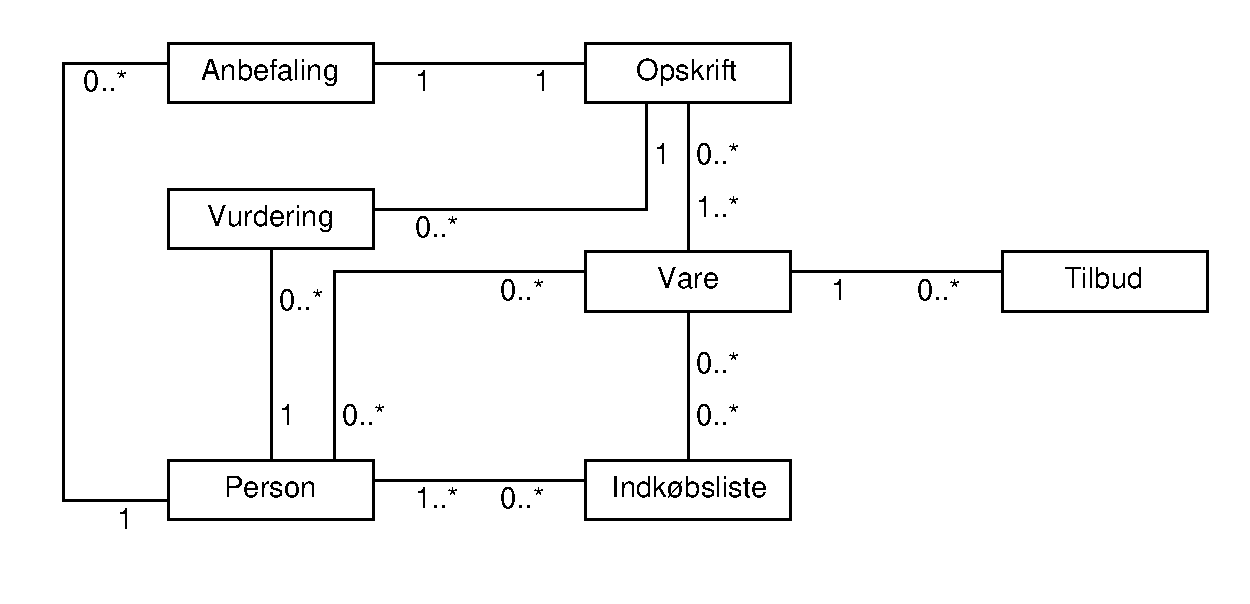
\includegraphics[scale=0.6]{images/Diagrams/klassediagram_model_simple.pdf}
	\caption{Klassediagram over problemområdet.}\label{figur:PDklasse}
\end{figure}

Klassediagrammet som ses på \myref{figur:PDklasse}, beskriver forholdet mellem de forskellige klasser som findes i problemområdet.
Diagrammets sammenhænge er dannet ud fra hændelsestabellen, og beskrivelserne af klasserne.\fxnote{Sørg for at denne model stemmer over ens med modellen vi ender ud med i programmet. I programmet kan vi så henvise til at denne model over klasserne blev brugt til at danne associationerne, imellem klasserne. Der er nemlig ingen henvendelse lige pt, og det kan helt klart bruges. Beskrivelsen nedenfor er næsten identisk med den man finder i Arkitektur - Søren}

Personer kan lave indkøbslister, disse indkøbslister kan være ejet og administreret af enten en eller flere personer.
En indkøbsliste kan bestå af nul til mange varer.
En vare kan være på tilbud i mere end en butik, og derfor have nul til mange tilbud.
En vare kan desuden indgå i en opskrift, og er derfor forbundet med nul til mange.
Desuden har opskrifterne en til mange varer på listen over ingredienser.
Varen kan også være tilføjet til overvågningslisten hos en person, så derfor har personer og varer en nul til mange relation på hinanden.
En person i problemområdet kan give hver opskrift en vurdering, derfor kan personen give nul til mange vurderinger.
En vurdering gives til en opskrift alene, imens en opskrift kan have mange vurderinger, eller ingen vurderinger.
Anbefalinger består af en opskrift, imens personen kan modtage nul til mange anbefalinger.

Ovenstående analyse vil hjælpe til at designe systemets implementering, først foretages dog en analyse af anvendelsesområdet, for at undersøge hvad der er muligt at foretage sig i systemet.

\section{Analyse af anvendelsesområdet}\label{sec:anvendelses}
Dette afsnit tager udgangspunkt i metoder fra ''Objektorienteret Analyse og Design'' og benytter disse til at analyserer anvendelsområdet, dette omfatter brug af systemet, funktioner i systemet samt grænsefladen der er tilknyttet.\citep{OOA&D2001} 
Afsnittet skal give et overblik over funktionaliteten af systemet, samt formidle hvordan brugeren interagere med systemet.

\subsection{Brug}
Denne del af analysen har til formål at fastlægge interaktion mellem systemet og aktører.
Dette gøres ved at identificere brugsmønstre for aktørerernes aktioner i systemet.
\subsubsection*{Aktører}
I dette IT-system er der blevet identificeret to aktører. 
Den første værende datakilden, eTilbudsavisens API, hvor tilbudende hentes fra og den anden værende de brugere, som benytter systemet.
For disse to aktører er der således udarbejdet en aktørtabel \myref{aktortabel}, der giver overblik over hvilke brugsmønstre der er, samt hvilke aktører der er relevante for disse.

\begin{table}[h]
\centering
    \colorlet{shadecolor}{gray!40}
    \rowcolors{1}{white}{shadecolor}
\begin{tabular}{rcc}
%\hline
				    & Bruger               		& eTilbudsavis  \\ \hline
Login               & \cmark                    & 		 		\\
Listehåndtering     & \cmark                    & 		 		\\
Søgning             & \cmark                    & 				\\
Indstil præferencer & \cmark                    & 				\\
Vurder opskrift     & \cmark                    &  	   			\\
Se anbefalinger     & \cmark                    & 				\\
Hent tilbud         &  						    & \cmark 		\\ \hline
\end{tabular}
\caption{Aktørtabel. Viser hvilke aktører er involveret i hvilke brugsmønstre}\label{aktortabel}
\end{table}

\subsubsection*{Bruger}

\textbf{Formål:} En person, som ønsker at bruge en eller flere af IT-systemets funktionaliteter, til at hjælpe med planlægning af mad og indkøb.

\textbf{Karakteristik:} Systemets brugere har meget varierende erfaring med IT-systemer, samt er bredt ud over mange forskellige aldersgrupper, majoriteten er dog mellem 18 - 30 år og har middel erfaring med IT.

\textbf{Eksempler:}Bruger A er en 21-årig universitetsstuderende, som for nyligt er flyttet hjemmefra. A har meget erfaring med IT, og bruger det dagligt til at navigere rundt på internettet. 
A har let ved at navigerer rundt i systemet og bruge dets funktionaliteter til at lave besparelser på det allerede lave budget, samt at undgå at få pasta med ketchup til aftensmad hver dag.

Bruger B er en 47-årig familiefar, der kun har smartphone, da det er arbejdstelefonen på givet af arbejdet. 
B benytter systemet til at handle ind på vej hjem fra arbejde, hvor indkøbslisten lavet af konen eller datteren bruges som guide i supermarkedet. 
B vil således gerne kunne tilgå listen fra telefonen, så der ikke er behov for at kører hjem og hente den på papirsformat.

\subsubsection*{eTilbudsavisen}

\textbf{Formål:} eTilbudsavisen har til formål at gøre tilbudsdata tilgængelig for systemet, dette sker igennem API.
Dette giver information om navnet på tilbudet, pris, periode, butik og meget andet.
Da dataene der hentes igennem API'et kan være af meget svingende kvalitet, filtreres det, så kun forståeligt tilbudsdata kommer igennem.

\textbf{Karakteristik:} eTilbudsavisen er pålidelig med dataene der sendes, kvaliteten af dataene kan dog svinge meget, og eTilbudsavisen tilbyder ingen fleksibilitet i dets arbejde, hvilket resulterer i noget ubrugeligt data som filtreres fra.

\textbf{Eksempel:} eTilbudsavisen gør 2.000 tilbud tilgængelig, heri er nogle på et format der ikke klargøre hvad der er på tilbud, men blot giver en række mærkenavne som er på tilbud.
En sådan uforståelig række bliver filtreret ud såvel som andre uforståelige tilbud, og systemet ender tilbage med 1.337 brugbare tilbud, der kan vises til brugeren.

\subsubsection*{Brugsmønstre}
For en yderligere beskrivelse af de funktionaliteter i systemet, som vedrører en given aktør, modelleres en række brugsmønstre, dette er de samme brugsmønstre som ses i aktørtabellen i \myref{aktortabel}. 
Hver enkelt af disse mønstre vil blive beskrevet igennem en brugsmønstrespecifikation. 
Det er ikke alle mønstre som ses på denne liste, nogle af disse er sammentrækninger af flere andre mønstre, som alene virker simple og repetitive at beskrive. 
Andre er udeladt da de ikke passer helt ind i en sammentrækning, men variationen fra det mønster og andre brugsmønstre ellers beskrevet, er så minimal, at mønstret er anset som værende ubetydeligt at beskrive.

\subsubsection*{Brugeridentifikation}
\textit{Brugsmønster:} Brugeridentifikation sker ved at en bruger logger ind i systemet.
Brugeren vil blive præsenteret for en side hvor, e-mail og password kan indtastes.
Herefter godkender eller afviser systemet den indtastede data og håndterer resultatet, enten ved at logge brugeren ind, eller ved at give en fejlbesked.
Alternativt kan brugeren oprette en ny konto i systemet, ved oplysning af navn e-mail og password.
Hvis du ikke er logget ind i systemet kan du ikke tilgå systemets funktionaliteter.

\textit{Objekter:} Person.

\textit{Funktioner:} Registrer bruger, Log ind, Log ud.

\subsubsection*{Listehåndtering}
\textbf{Brugsmønster:} Dette brugsmønster dækker over indkøbslisten såvel som overvågningslisten.
Brugeren kan inden for listens brugsmønstre tilgå funktionaliteterne i vilkårlig rækkefølge, givet der er oprettet en liste på forhånd.
En bruger kan oprette, dele og slette sine egne indkøbslister.
Hvis en liste er delt med andre og prøver at slette denne, forlader brugeren listen frem for at slette den.
Overvågningslisten på den anden hånd, eksisterer altid og kan hverken oprettes eller slettes.
Brugeren kan på begge lister tilføje eller fjerne en vare.
Varerne på overvågningslisten er varer som brugeren er interesserede i at få tilbud om.
Når en vare på denne liste kommer på tilbud modtager brugeren en notifikation derom.
Ved indkøbslisten er der tre funktionaliteter til at tilføje ting til listen.
Man kan tilføje ingredienser fra en opskrift.
Ydermere kan en bruger aftjekke eller fjerne varer fra listen.

\textbf{Objekter:} Indkøbsliste, Overvågningsliste, Varer, Tilbud, Personer, Opskrifter.

\textbf{Funktioner:} Opret liste, Fjern Indkøbsliste, Tilføj til liste, Fjern fra liste, Aftjek på indkøbsliste, Del liste, Forlad Indkøbsliste.

\subsubsection*{Søgning}
\textbf{Brugsmønster:} Brugeren kan søge efter varer, hvorefter systemet filtrerer efter søgestrengen for at finde relevante resultater.
Dette brugsmønster benyttes flere steder, både til at søge på tilbud til sine varer, såvel som opskrifter.


\textbf{Objekter:} Vare, Tilbud, Opskrifter.

\textbf{Funktioner:} Søg efter tilbud, Søg efter opskrifter.

\subsubsection*{Tilpas præferencer}
\textbf{Brugsmønster:} 
Brugere i systemet har mulighed for at fravælge madvarer eller butikker, som vises i programmet.

\textbf{Objekter:} Varer.

\textbf{Funktioner:} Sæt Præferencer, Filtrer efter præferencer.

\subsubsection*{Opskrifts håndtering}
\textbf{Brugsmønster:}
Brugeren kan interagere med opskrifter på forskellig vis. 
Som bruger har man mulighed for at oprette, klone, ændre, slette og vurdere opskrifter.
Når en opskrift oprettes vil brugeren bedes tilføje instruktioner, tid og ingredienser.
En bruger vil have mulighed for at ændre i sine egne opskrifter, og ligeledes kunne kopiere andres opskrifter og derefter tilføje ændringer i disse.
Fra ingredienslisten på en opskrift kan brugerne tilføje en eller flere varer til deres indkøbslister, samt skalere ingredienslisten til et bestemt antal personer, så brugerne får købt den rigtige mængde.
Brugerne har også mulighed for at vurdere opskrifter, ud fra brugerens vurderinger, vil systemet anbefale nye opskrifter til brugeren.

\textbf{Objekter:} Opskrift, Vurdering, liste af vurderinger, varer, indkøbsliste.

\textbf{Funktioner:} Se opskrift, oprette opskrift, ændre opskrift, klone opskrift, vurder opskrift, tilføj vare til liste, skalering af opskrift, slette opskrift.

%\subsubsection*{Vurder}
%\textbf{Brugsmønster:}
%Efter en opskrift er vurderet, kan andre brugere se den gennemsnitlige vurdering af en opskrift, og de brugere som har vurderet opskrifter, vil få anbefalet opskrifter som ligner.
%
%\textbf{Objekter:} Opskrift, Vurderinger, Liste af vurderinger.
%
%\textbf{Funktioner:} Vurder opskrift.

\subsubsection*{Se anbefalinger}
\textbf{Brugsmønster:} Brugeren kan se foreslåede opskrifter ud fra tidligere vurderede opskrifter.

\textbf{Objekter:} Opskrift, Vare.

\textbf{Funktioner:} Send anbefaling.

\subsubsection*{Hent tilbud}
\textbf{Brugsmønster:} Dette brugsmønster igangsættes af systemet, der periodisk henter tilbud fra eTilbudsavis og gemmer dem i systemet.

\textbf{Objekter:} Tilbud.

\textbf{Funktioner:} Hent tilbud.


\subsubsection{Funktioner}

I dette afsnit beskrives funktionerne der skal bruges for at kunne håndtere hændelserne fra problemområdet, og brugsmønstrene beskrevet ovenfor. 
Der findes fire typer funktioner: Aflæsnings-, opdaterings-, beregnings-, og signaleringsfunktioner.\citep{OOA&D2001}
Først identificeres funktionerne, hvorefter der gives en kategori til funktionerne, og en bedømmelse af deres kompleksitet. Herefter gives en kortfattet beskrivelse af funktionen hvor dette er tilstrækkeligt, ellers gives en dybere beskrivelse.

\begin{table}[H]
  \centering
    \colorlet{shadecolor}{gray!40}
    \rowcolors{1}{white}{shadecolor}
      \begin{tabular}{l|lllll}
      %\hline
      \textbf{Funktioner}			& {Kompleksitet}	& {Kategori}  	\\ \hline
      Log ind						& Medium			& Beregning, Opdatering		\\
      Log ud						& Simpel			& Opdatering	\\
      Registrer bruger				& Simpel			& Opdatering	\\
      Tilføje varer til lister		& Simpel       		& Opdatering	\\ 
      Fjerne varer fra lister		& Simpel       		& Opdatering	\\ 
      Oprette og slette lister		& Simpel       		& Opdatering	\\ 
      Dele lister					& Medium       		& Opdatering	\\ 
      Søgning på tilbud for varer   & Medium     		& Beregning		\\ 
      Sætte præferencer				& Simpel       		& Opdatering	\\ 
      Filtrere for præferencer		& Kompleks     		& Beregning		\\ 
      Give vurdering				& Simpel       		& Opdatering	\\ 
      Sende anbefaling				& Meget kompleks	& Aflæsning, signalering, beregning		\\ 
      Meddele tilbud på varer		& Medium      		& Signalering	\\ 
	  Se opskrifter					& Simpel       		& Aflæsning		\\ 
	  Se tilbud						& Simpel       		& Aflæsning		\\ 
      Hente tilbud					& Simpel	       	& Opdatering	\\           
    \end{tabular}
  \caption{Funktionstabel. Viser de forskellige funktioner der skal bruges, samt deres kompleksitet og kategori.}\label{tabel:functionstable}
\end{table}

\textbf{Log ind:} Her bliver sendt brugerinformationer, som verificeres med brugerne registreret i systemet. 
Hvis dette fuldføres, opdateres modellen således brugeren er registreret som værende logget ind.

\textbf{Log ud:} Brugeren der før var logget ind, opdateres til at være logget ud.

\textbf{Registrer bruger:} En ny bruger sender sine brugerinformationer, og et nyt login oprettes i modellaget.

\textbf{Tilføje varer til lister:} Denne funktion skal tilføje et objekt af vare klassen til en indkøbsliste, eller en overvågningsliste.

\textbf{Fjerne varer fra lister:} Funktionen her skal så fjerne disse objekter igen.

\textbf{Oprette og slette lister:} Denne funktion bruges når en indkøbsliste skal oprettes således man kan tilføje varer til denne.

\textbf{Dele lister:} Skal opdatere modellen således en anden bruger kan tilgå samme indkøbsliste som brugeren der deler sin liste. 

\textbf{Søgning på tilbud for varer:} Søger efter tilbud som passer til varen der søges for.

\textbf{Sætte præferencer:} Funktionen skal sætte forskellige præferencer som vælges af brugeren, således brugerens oplevelse rettes efter brugerens præferencer.

\textbf{Filtrere for præferencer:} Funktionen skal findes i to udgaver. Der skal være filtrering i forhold til præferencer for både tilbud, og opskrifter.

\textbf{Give vurdering:} Funktionen skal modtage en vurdering fra brugeren og gemme denne i modellaget.

\textbf{Sende anbefaling:} Funktionen her er meget kompleks da der indgår mange forskellige typer handlinger. 
Brugerne har vurderet forskellige opskrifter, og der beregnes en anbefaling ud fra disse.
Når anbefalingen er lavet skal den gives eller signaleres til brugeren.

\textbf{Meddele tilbud på varer:} Når en varer på overvågningslisten kommer på tilbud sender denne funktion et signal til brugeren derom.

\textbf{Se opskrifter:} Funktionen skal hente opskrifterne fra modellaget.

\textbf{Se tilbud:} Funktionen henter tilbudene fra modellaget.

\textbf{Hente tilbud:} Denne funktion henter tilbud, vha. API'et fra eTilbudsavis, disse skal derefter gemmes i modellaget.

Denne analyse af funktionerne hjælper med at danne et overblik over hvilke funktionaliteter der skal designes, samt hjælper det til at stille krav til det endelige produkt.

\section{Kravspecifikation}\label{sec:krav}

På baggrund af analysen af problemområdet, anvendelsesområdet og interviewene beskrevet i  \myref{section:interview2} kan der nu opstilles krav til systemet, samt hvad det skal kunne.
Følgende user stories er baseret på brugsmønstrene og funktionerne fra \myref{sec:anvendelses}, samt svarene fra de interviewede.
Som nævnt i \myref{chapter:Metode} benytter vi user stories til at formulere kravspefikationen, da vi benytter Scrum.
\begin{enumerate}
	\item Som en bruger vil jeg kunne oprette indkøbslister.
	\item Som en bruger vil jeg kunne tilføje varer til min(e) indkøbsliste(r).
	\item Som en bruger vil jeg kunne se tilbud.
	\item Som en bruger vil jeg kunne se tilbudsvarer jeg har valgt, deres pris, butik og dato på indkøbslisten.
	\item Som en bruger vil jeg kunne aftjekke en vare fra indkøbslisten.
	\item Som en bruger vil jeg kunne overvåge specifikke vare, og få en notifikation når disse varer kommer på tilbud.
	\item Som en bruger vil jeg kunne finde opskrifter.
	\item Som en bruger vil jeg gerne logge ind.
	\item Som en bruger vil jeg kunne finde opskrifter ud fra anbefalinger til mig.
	\item Som en bruger vil jeg kunne vurdere opskrifter jeg har prøvet.
	\item Som en bruger vil jeg kunne indstille mine præferencer.
	\item Som en bruger vil jeg kunne ekskludere tilbud fra butikskæder som ikke er relevante for mig.
	\item Som en bruger vil jeg kunne dele min indkøbsliste med andre.
	\item Som en bruger vil jeg kunne søge på varer, og finde deres tilbud.
	\item Som en bruger vil jeg kunne tilføje ingredienser for en opskrift til min indkøbsliste.
	\item Som en bruger vil jeg kunne tilgå min indkøbsliste fra min smartphone.
	\item Som en bruger vil jeg kunne skalere opskrifterne til et valgt antal personer.
\end{enumerate}

Disse user stories vil blive designet og implementeret i systemet.
Desuden stilles der yderligere krav til projektet og systemet, bl.a. fra funktionaliteter fundet i \myref{subsec:funktioner}, og fra studieordningen.

\subsection{Krav til systemet}
\begin{enumerate}
\item Der skal benyttes C\# til programmering af systemet.
\item Systemet skal kunne tilgås via forskellige enheder, og gemme information fra enhed til enhed.
\item Systemet skal benytte aktuelle tilbud fra diverse dagligvarebutikker.
\item Systemet skal kunne modtage feedback på de opskrifter brugerne prøver.
\item Systemet skal kunne anbefale opskrifter på baggrund af:
\begin{enumerate}
	\item Madvaner (varieret kost).\fxnote{Dette krav er ikke overholdt, og har aldrig været med i vores overvejelser til udviklingsprocess}
	\item Bedømmelse på opskrift.
\end{enumerate}
\item Systemet skal kunne fjerne forslag om eksempelvis kød til vegetarer ud fra præferencer.
\end{enumerate}

\subsection{Krav til UI (brugergrænseflade)}
\begin{enumerate}
	\item Systemets UI skal være på dansk.
	\item Systemet skal kunne anvendes på forskellige enheder
	\item Systemets UI skal være responsivt og tilpasse sig den anvendte platform.
	\item Brugerne skal synes det er nemt at skabe sig overblik over systemet og navigering heri.
\end{enumerate}

Alle kravene i dette afsnit vil blive taget i betragtning, under design og implementering af systemet.
Slutteligt i rapporten konkluderes der på hvor vidt disse krav er opfyldt, og desuden vil der udføres endnu en række interviews med brugere for at teste deres tilfredsstillelse med systemet.
I de følgende afsnit vil udviklingsprocessen yderligere beskrives, samt designet og implementationerne af løsninger til kravene stillet i dette afsnit.



%\makeatletter\@openrightfalse
%\let\cleardoublepage\clearpage
\part{Udvikling}
\chapter{Udvikling}
\fixme{indledning her - morten}
\subsection{MVC-mønsteret}\label{MVC}
Et af de standardiserede design mønstre, som bruges af mange udviklere er MVC-mønsteret - som står for \textit{Model-View-Controller}.
MVC-mønsteret har til formål, at dele systemet op i tre komponenter, nemlig \textit{Model}, \textit{View} og \textit{Controller}.
Denne segregering adskiller således ''forretnings-logik'', ''input-logik'' og ''UI-logik'', og gør herved systemet mere fleksibelt, samt fremmer muligheden for at udvikle parallelt på de forskellige komponenter.
Dette kan være nyttigt i udviklingen af systemet, men også efter udgivelsen, idet blandt andet ''UI-logik''kan blive ændret oftere end for eksempel ''forretnings-logik''.
Opdelingen hjælper også til at skabe overblik over koden, og gør det nemmere at udføre tests på systemet. \citep{MVC_Overview}

\begin{wrapfigure}{r}{0.4\textwidth}
	\vspace{-20pt}
	\begin{center}
		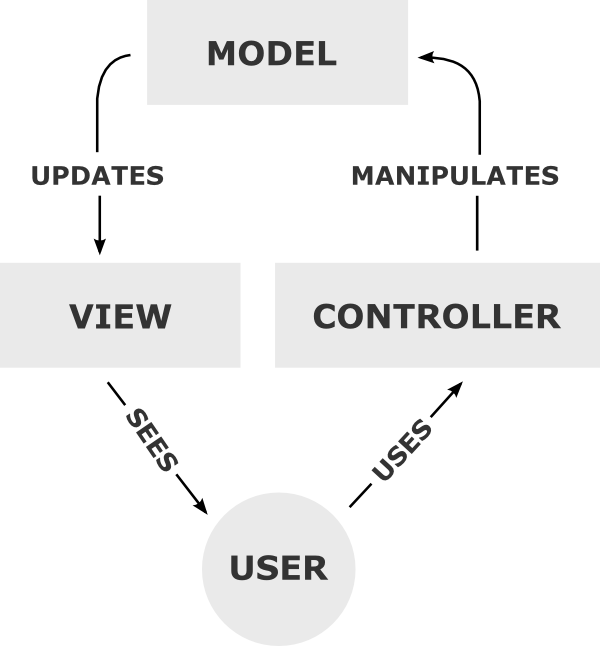
\includegraphics[width=0.38\textwidth]{images/Images/mvc.png}
	\end{center}
	\vspace{-20pt}
	\caption{MVC-mønsteret}
	\vspace{-20pt}
\end{wrapfigure}


Nedenfor beskriver vi de tre komponenter.

\textbf{Model}\\
De objekter, der udgør model-laget skal indeholde den før omtalte ''forretnings-logik'', samt alle data der skal modelleres i systemet.
Dataen, i form af objekter, gemmes oftest i en database eller fil, og er helt skjult for brugeren i den forstand, at al repræsentation af modellen foregår igennem view-delen af MVC-mønsteret.

\textbf{View}\\
Der er igennem forskellige views, at brugeren får præsenteret brugergrænsefladen - også kaldet UI(user-interface).
Derfor giver det også mening, at placere ''UI-logikken'' i denne del af MVC-mønsteret.
Typisk bliver et views indhold genereret ud fra data fra en model.
Et eksempel på dette ville være visning af en liste af objekter ud fra en model, der indeholder netop en liste.

\textbf{Controller}\\
Når det kommer til interaktionen mellem brugeren og systemet, er det controlleren der påtager sig opgaven.
Derfor er det også i de forskellige controllerere, at vi finder ''input-logikken''. Her bestemmes ud fra input fra brugeren hvilke data der skal arbejdes med i hvilken model og også hvilket view, der skal præsenteret for brugeren. Med dette kan vi også se, at viewet ikke indeholder nogenb logik og al manipulation af data altså foregår gennem controller komponenten.

\section{Anvendte teknologier}
I dette afsnit beskrives teknologierne, gruppen har valgt at anvende til udviklingen af projektet.
Disse teknologier er valgt for at opfylde studieordningen, hvor C\# skulle være det anvendte programmeringssprog, og desuden for at behjælpe i at opfylde kravene stillet i \myref{sec:krav}.

\subsection{Bootstrap}
``Bootstrap'' er navnet på et front-end web udviklings framework, oprindeligt udviklet af Twitter til eget brug, men senere frigivet som open source. 
Bootstrap er i følge dem selv ``[...] the most popular HTML, CSS, and JS framework for developing responsive, mobile first projects on the web.'' \cite{GETBOOTSTRAP}
Som de selv skriver så giver Bootstrap mulighed for at bruge den samme teknologi på tværs af enheder, dette gør det nemmere for udviklere at give brugeren en mere konsistent oplevelse.
Et af de vigtigste koncepter bag Bootstrap er at hver side består af et gitter som er 12 kolonner. 
På den måde er det nemt at bestemme bredden på et givent element, ved at indgrænse det til en del af sidens bredde, dette vil også automatisk forsøge at skalere sig til en mobil enhed. 
Anvendelsen af Bootstrap sker når man påklæder sine HTML elementer med de givne CSS klasser som Bootstrap udgiver. 
Det er herunder muligt at anvende flere klasser på samme element, samt den samme klasse på tværs af forskellige HTML elementer. 
Dette bidrager til at øge konsistensen i layoutet.
JavaScript bruges i Bootstrap til at animere elementer på siden.
 
Dette øger brugerens interaktion, og bringer Bootstraps elementer til live. \cite{GETBOOTSTRAP}

\subsection{ASP.NET MVC 5}
``ASP.NET MVC 5'' er navnet på Microsofts open source implementering af MVC mønstret (beskrevet i \myref{MVC}). 
ASP.NET MVC er baseret på grundtanken om at opdele de forskellige logiske lag i applikationen: Modellen (``business layer''), Viewet (``display layer'') og Controlleren (``input kontrol''). 
Brugen af ASP.NET giver mulighed for at bruge den såkaldte ``Razor syntax'', som er en del af ``ASP.NET Razor view engine''.
Den gør det muligt at anvende C\#-kode (Eller Visual Basic .NET) i front-enden, til at genere dynamiske hjemmesider. 
Disse udtryk evalueres serverside ved runtime, derfor er alle datatyperne dynamiske, og ikke typesikre, det antages altså ved compiletime at alle operationer er mulige på objekter at typen ``dynamic''. \footnote{http://msdn.microsoft.com/en-us/library/dd264736.aspx}

\subsection{Entity Framework}
Entity Framework (``EF'') er et Object-relational mapping (``ORM'') framework til .NET frameworket, udviklet af Microsoft, og er databasen der bruges i projektet. \citep{EF} 
EF er valgt til dels grundet at det er muligt at udvikle ``Code-first'', hvilket vil sige at udvikleren først skriver modellen som klasser, hvorefter databasestrukturen kan opbygges. 
Der understøttes komplicerede relationer såsom mange-til-mange og en-til-mange, ved brug af en relationsdatabase, som er en tabel der kæder 2, eller flere, informationer sammen på tværs af tabeller.

\section{Arkitektur}
Dette afsnit beskriver arkitekturen der benyttes i implementationen for systemet.
Først gennemgås design mønsteret der benyttes, derefter systemets klasser, samt dets komponenter.

Nogle komponenter har vi valgt at benytte, ASP.NETs indbyggede programdele.
Vi benytter os af en færdig login løsning, der er tilgændeligt i ASP.NET teknologien (se eventuelt \myref{apsnet}).
Dette har vi valgt, da vi har vuderet at login ikke er en central problemstilling i forhold til studieordningen og projektets mål.
Dette tillader os at bruge mere tid på andre dele af programmet, som vi finder mere relavante i forhold til de opstillede mål.
Denne implementation er udført for at opfylde user story 10.

\subsection{MVC-mønsteret}\label{MVC}
Et af de standardiserede design mønstre, som bruges af mange udviklere er MVC-mønsteret - som står for \textit{Model-View-Controller}.
MVC-mønsteret har til formål, at dele systemet op i tre komponenter, nemlig \textit{Model}, \textit{View} og \textit{Controller}.
Denne segregering adskiller således ''forretnings-logik'', ''input-logik'' og ''UI-logik'', og gør herved systemet mere fleksibelt, samt fremmer muligheden for at udvikle parallelt på de forskellige komponenter.
Dette kan være nyttigt i udviklingen af systemet, men også efter udgivelsen, idet blandt andet ''UI-logik''kan blive ændret oftere end for eksempel ''forretnings-logik''.
Opdelingen hjælper også til at skabe overblik over koden, og gør det nemmere at udføre tests på systemet. \citep{MVC_Overview}

\begin{wrapfigure}{r}{0.4\textwidth}
	\vspace{-20pt}
	\begin{center}
		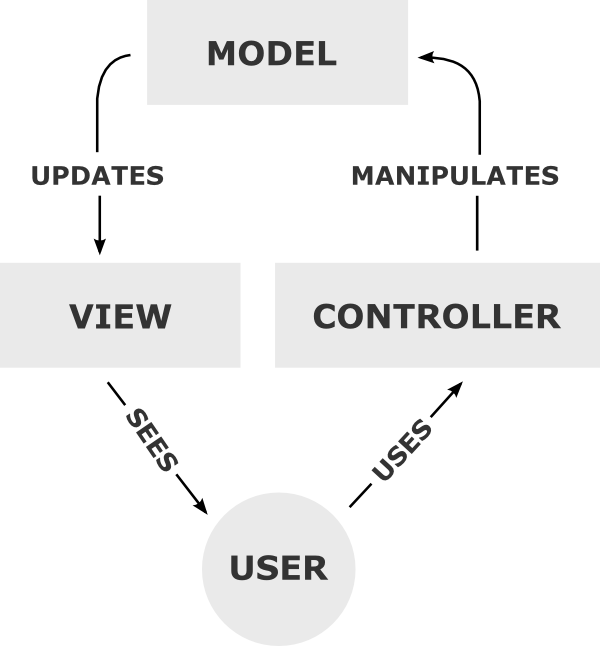
\includegraphics[width=0.38\textwidth]{images/Images/mvc.png}
	\end{center}
	\vspace{-20pt}
	\caption{MVC-mønsteret}
	\vspace{-20pt}
\end{wrapfigure}


Nedenfor beskriver vi de tre komponenter.

\textbf{Model}\\
De objekter, der udgør model-laget skal indeholde den før omtalte ''forretnings-logik'', samt alle data der skal modelleres i systemet.
Dataen, i form af objekter, gemmes oftest i en database eller fil, og er helt skjult for brugeren i den forstand, at al repræsentation af modellen foregår igennem view-delen af MVC-mønsteret.

\textbf{View}\\
Der er igennem forskellige views, at brugeren får præsenteret brugergrænsefladen - også kaldet UI(user-interface).
Derfor giver det også mening, at placere ''UI-logikken'' i denne del af MVC-mønsteret.
Typisk bliver et views indhold genereret ud fra data fra en model.
Et eksempel på dette ville være visning af en liste af objekter ud fra en model, der indeholder netop en liste.

\textbf{Controller}\\
Når det kommer til interaktionen mellem brugeren og systemet, er det controlleren der påtager sig opgaven.
Derfor er det også i de forskellige controllerere, at vi finder ''input-logikken''. Her bestemmes ud fra input fra brugeren hvilke data der skal arbejdes med i hvilken model og også hvilket view, der skal præsenteret for brugeren. Med dette kan vi også se, at viewet ikke indeholder nogenb logik og al manipulation af data altså foregår gennem controller komponenten.


\subsection{Program komponenter}\label{subsec:komp}

Der kan dannes forskellige komponenter i programmet ud fra de user stories der blev opgivet på \myref{sec:krav}.
Disse kan ses på \myref{figure:komp}.
Figuren viser hvordan de forskellige user stories kan deles op i komponenter, og hvordan disse komponenter afhænger og bruger hinanden som beskrevet ud fra vores user stories.

\begin{figure}
	\vspace{-20pt}
	\begin{center}
		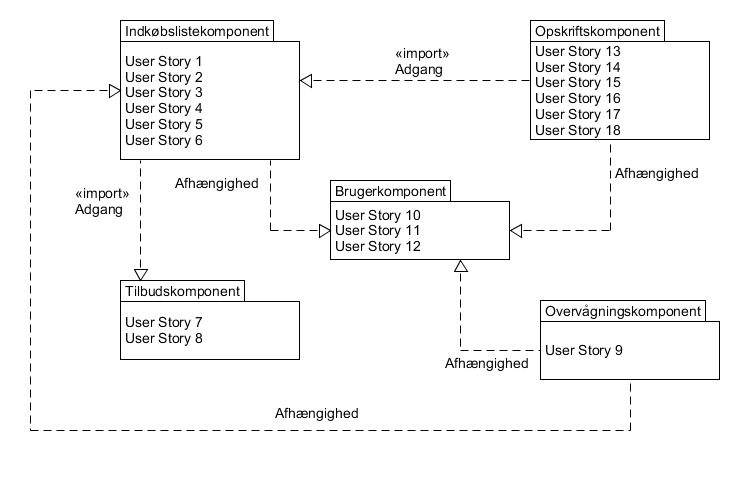
\includegraphics[scale=0.6]{images/Diagrams/Komponenter.png}
	\end{center}
	\vspace{-20pt}
	\caption{UML 2 Komponent diagram }
	\label{figure:komp}
	\vspace{-20pt}
\end{figure}

\textbf{Indkøbslistekomponentet} står for at lave indkøbslister, og tilføje varer og tilbud til disse.
Tilbudene skal importeres fra \textbf{tilbudskomponentet}, for at lave koblingen imellem varerne og tilbud.
Det er afhængigt af \textbf{brugerkomponentet} da indkøbslisterne hører til en bruger for at danne personlige lister. Brugerkomponentet er ansvarlig for alt der har med en bruger at gøre. Det indebærer at registrere hvem der er logget på, håndtere brugerens personlige indstillinger. Det er altså dette komponent der sørger for den personlige oplevelse på hjemmesiden.

\textbf{Opskriftskomponentet} er afhængig af brugerkomponentet, da det er brugerene i systemet der tilføjer opskrifter, samt giver opskrifterne en rating.
Dog er det opskriftskomponentet der står for dette, men det skal dog vide hvem der er logget ind på hjemmesiden.
Der er en adgang her fra til indkøbslisterne for at kunne tilføje ingredienser fra opskrifterne til indkøbslister.

\textbf{Overvågningskomponentet} står for at overvågningen af tilbud for en specifik varer kan foregå.
Der dannes en afhængighed herfra og til indkøbslistekomponentet da overvågningslisten gør brug af de metoder som der stilles til rådighed i dette komponenet, såsom tilføje varer, og finde tilbud.


\subsection{Klassediagram}
For at illustrere modellaget i vores MVC-mønster, har vi produceret et klassediagram (se \myref{diagram:klassediagram} nedenfor) i UML, der simplificerer strukturen.
Det skal bemærkes, at klasserne og felterne er på dansk i diagrammet, og på engelsk i selve koden af programmet. \fxfatal{Der er ingen adgangsting på dette, private, protected, public etc. Er det bevist? Derudover er det ikke klart hvilken datatype hvert felt er, også om det er en liste eller ej. - Troels - Fikser figuren senere - Søren}

\begin{figure}[H]
\centering
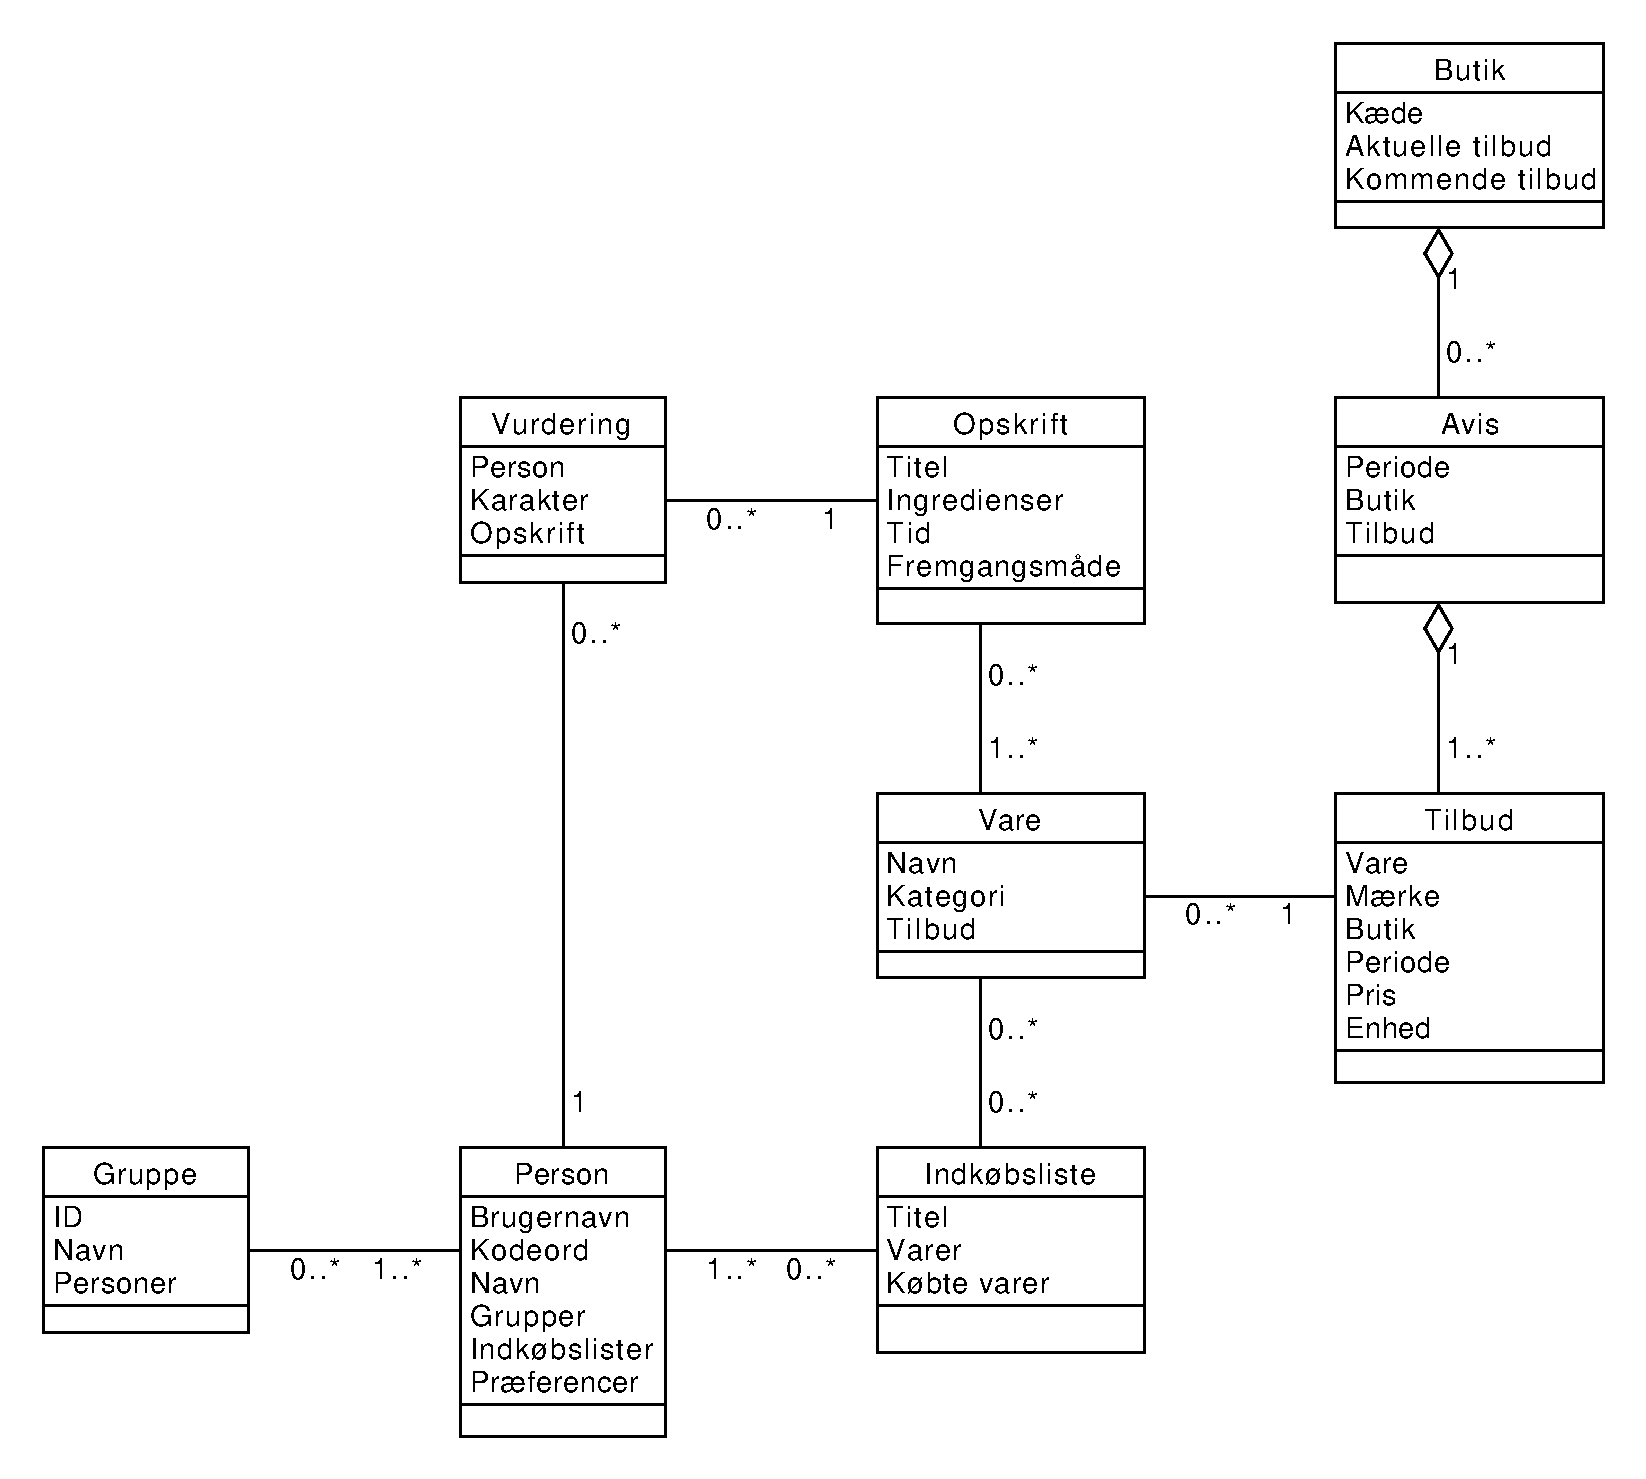
\includegraphics[width=0.8\linewidth]{/Diagrams/klassediagram_model_expanded_implemented.pdf}
\caption{UML klassediagram for modellaget i MVC-mønsteret}\label{diagram:klassediagram}
\end{figure}

\subsection{Klasserne}
Vi vil gennemgå klasserne, der optræder i klassediagrammet, og beskrive deres relationer samt deres felter.

\fxnote{Indsæt figur for hver enkelt klasse.}

\subsubsection{Person}
Person-klassen i modellen, er den der holder styr på brugeren og dennes basale attributter - herunder brugernavn, kodeord og kaldenavn.
Ydermere er det vigtigt, at objektet kan indeholde informationer om personens madpræferencer og vurderinger af opskrifter; dette er med til at give person-klassen en mere intim vinkel, og så at sige bedre afspejle den virkelige person, samt fungere som grundlag for anbefaling af opskrifter.
Det er naturligvis også vigtigt for et program, der omhandler bl.a. indkøbslister, at holde styr på en persons indkøbslister og lignende.
Til dette har person-klassen to felter der hedder henholdsvis, grupper og indkøbslister.
Begge felter er lister\fxfatal{Som nævnt tidligere er dette ikke klart fra diagrammet. - Troels}, der holder styr på personens relationer til netop grupper og indkøbslister - En person kan altså have relationer til flere grupper og flere indkøbslister, hvilket også kan ses ud fra de indtegnede relationer i klassediagrammet.


\subsubsection{Indkøbsliste}
Indkøbslister repræsenteres i systemet som klassen ´´Indkøbsliste'', og indeholder ID, titel og to lister med varer.
ID'et garanterer, at alle indkøbslister er unikke og kan skelnes fra hinanden på systemsiden.
Indkøbsliste-klassen har et titel felt, så brugeren også kan navigere mellem forskellige instanser.
De to lister af varer, holder styr på henholdsvis; varer som bliver tilføjet til listen, og varer som har været tilføjet men er blever markeret som købt.
Der er således kun styr på ''overstregede'' varer - altså dem der er købt, og ikke varer som bliver slettet fra listen.
En indkøbsliste kan godt eksisterer uden varer, idet brugeren skal kunne oprette lister, inden der er taget stilling til, hvilke varer der skal bruges.
Indkøbsliste har kun relation til en gruppe, men kan godt have relationer til flere personer.\fxnote{Findes der stadig to lister - Bruger vi dem ?}

\subsubsection{Vare}
Vare-klassen indeholder tre felter: Et navn på varen, som er generisk, for eksempel ''Letmælk'' og ''Cola'' istedet for ''Arla Letmælk'' og ''Pepsi''; en kategori, der beskriver varen, for eksempel ''Mejeri'' eller ''Pålæg''; og en liste over tilbud, der holder styr på, hvis og hvor varen eventuelt er på tilbud.
En vare behøver ikke være på en indkøbsliste eller opskrift for at eksistere \fixme{kan det passe?}, og kan have relationer til nul til mange tilbud.

\subsubsection{Tilbud}
Et tilbud som instans af Tilbud-klassen, indeholder felter der beskriver: Varen, mærket, hvilken butik tilbuddet befinder sig i, hvilken periode tilbuddet gælder i, prisen på tilbudet, og hvilken enhed/mængde tilbudet er i.
Ud fra disse atributter er det muligt at identificere tilbudet, og brugeren kan tage stilling til, om det er relevant.


\subsubsection{Opskrifter}
\lipsum[1]

\subsubsection{Vurdering}
\lipsum[1]


\section{eTilbudsavis API}\label{api}
I dette afsnit beskrives først teori om hvad et API er, og hvordan sådan et er struktureret.
Herefter gennemgås design og implementering for brug af eTilbudsavis' API samt motivationen for at bruge API'en. 
Til sidst vil der blive konkluderet på API'ens betydning for projektet.

User story 7 fortæller at man skal kunne se tilbud.
API'et gør det muligt at indhente infomation om butikker og deres tilbud.
Dette API udbydes af den danske virksomhed eTilbudsavis.dk, og er af typen REST.

\subsection{Teori}
Representational state transfer (REST) er en arkitektur anvendt over HTTP(S) standarden. 
I forbindelse med eTilbudsavisen anvendes der HTTP status koder, som signalerer hvorvidt en given forespørgsel er godkendt, afvist eller lign.

\subsubsection{API-Kald}
For at kommunikere med API'et skal der konstrueres en forespørgsel.
Inden for REST, bruges der de fire mest almindelige HTTP metoder, som er POST, GET, PUT og DELETE.
Disse fire metoder findes tilsvarende i CRUD som: CREATE, READ, UPDATE, DELETE.

\textbf{GET}
returnerer data, typisk som JSON eller XML og med HTTP svarkoden 200 (OK).
eTilbudsavis' API sender JSON.
Svarer til READ i CRUD.

\textbf{POST}
bruges til at oprette nye ressourcer.
Svarer til CREATE i CRUD.

\textbf{PUT}
bruges til at opdatere information, eksempelvis til at forlænge en session.
Svarer til UPDATE i CRUD.

\textbf{DELETE}
bruges til at fjerne ressourcer.
Svarer til DELETE i CRUD.

\subsection{Design}
eTilbudsavis' API er kun et halv-offentligt API, dvs. at man skal have en API-nøgle (``APIKEY'') og dertilhørende hemmelighed (``Secret''), som vi har modtaget eTilbudsavis.
API'en er placeret på \textit{https://api.etilbudsavis.dk/v2/}. \citep{eTilAPI}

For at kommunikere med API'en fra C\#-kode anvendes værktøjet RestSharp. RestSharp er en simpel REST og HTTP API klient for et .NET miljø. \citep{RestSharp}
For at kunne bruge informationen laves der en klasse, som svarer til det JSON som API'en sender tilbage.

\subsection{Vurdering}\label{api:skoddata}
Vi har valgt at benytte et API, især eTilbudsavis' API, da det giver os muligheden for at arbejde med og vise faktiske tilbud.
Der er dog fundet visse ulemper ved, at vi benytter os af eTilbudsavis' API.
Det data, vi modtager, begrænser os fra at udvikle flere funktioner, da det f.eks. ikke indeholder: information omkring mængde tilbud, kategori-inddeling eller forekomster af allergener i varerne. 
Dette er funktioner, vores testpersoner har adspurgt. 
Hvis disse tre attributter havde været tilstede, ville systemet for eksempel være i stand til at frasortere tilbud, der indeholder spor af jordnødder eller lignende, hvis den pågældende bruger eksempelvis er allergisk overfor jordnødder. 
Ligeledes ville det med kategori-inddeling være muligt at sortere mere intuitivt i tilbud, og information om grupperede tilbud ville give systemet mulighed for at præsentere visse tilbud bedre for brugeren, så der ikke opstår forvirring.

\subsection{Implementering}
Denne implementering er en del af controlleren: \class{OfferController.cs}, i metoden \class{ImportOffers}.
\subsubsection{Session}
For at kunne bruge API'et skal man først oprette en session.
En session består af en API-nøgle, den tilsvarende hemmelighed (Secret), en token og en signatur.
Har man en API-nøgle kan man kalde API'et sessions og få en token.
Den token kan man kombinere med sin hemmelighed og generere SHA-256 hashen af dette, som er signaturen, der brugers til at underskrive requests.

Eksempelvis vil API-kaldet, som opretter en session returnere:
\begin{lstlisting}[language=json,firstnumber=1,caption={POST til sessions API'et med APIKEY'en},label=apilst1]
{
    "token": "00hdcx7fnysn6541",
    "expires": "2013-03-03T13:37:00+0000",
    "user": null,
    "provider": null,
    "permissions": {
        "guest": [
            "api.public",
            "api.users.create"
        ]
    }
}
\end{lstlisting}

Dette svar kan oversættes til en klasse i C\#, som har tilsvarende felter, så den kan indlæses med RestSharp som vist i \myref{lst:session}.

\begin{lstlisting}[caption=C\#-kode som opretter en RestClient og anvender den til at oprette et objekt med felter som svarer til JSON dataet givet fra API'en, label=lst:session]
/* [...] */
/* Create a RestClient*/
var client = new RestClient("https://api.etilbudsavis.dk");

/* Initiate the first request to get a session */
var SessionRequest = new RestRequest("v2/sessions", Method.POST);
SessionRequest.AddParameter("api_key", Global.Apikey);

/* Map the response to the class "Session" */
IRestResponse<Session> response2 = client.Execute<Session>(SessionRequest);

/* Save the response in an object */
Session sessionobj = response2.Data;

/* Generate a signature and set it to the global variable */
Global.Signature = EncryptionHelper.SHA256(Global.Secret + Global.SessionToken);
/* [...] */
\end{lstlisting}
Efter eksekveringen af denne kode vil der være et objekt af datatypen \class{Session} kaldet \class{sessionobj}, som indeholder de samme felter som givet i JSON i \myref{apilst1}; derudover er signaturen, en SHA256 hash af hemmeligheden og sessiontokenen, (\class{Global.Signature}) også beregnet og gemt.

\subsubsection{Indlæsning af tilbud}
API'ets anvendelse i programmet er at indhente aktuelle tilbud.
For at kunne modtage tilbud skal der konstrueres et request, som minder om det vist i \myref{lst:session}, men anmoder tilbud.
Der er en øvre grænse sat af eTilbudsavis på, at maksimalt 100 tilbud kan hentes ad gangen, da der vil skulle hentes mere end 100 tilbud ad gangen, er det nødvendigt at fortage flere anmodninger.
Derfor bruges en \class{do..while} løkke som gentages, så længe der returneres 100 tilbud fra API'et, denne er vist i \myref{apiofferscs}.

\begin{lstlisting}[caption={C\#-kode som anvender ``/v2/offers'' delen af API'et til at hente tilbud.}, label=apiofferscs]
/* [...] */
var listofApiOffers = new List<ApiOffer>();
do {
    var nextOffersRequest = new RestRequest("v2/offers", Method.GET);
    nextOffersRequest.AddParameter("r_lat", Global.Latitude);
    nextOffersRequest.AddParameter("r_lng", Global.Longitude);
    nextOffersRequest.AddParameter("r_radius", Global.Radius);
    nextOffersRequest.AddHeader("X-Token", Global.Session.Token);
    nextOffersRequest.AddHeader("X-Signature", Global.Session.Signature);
    nextOffersRequest.AddParameter("limit", "100");
    nextOffersRequest.AddParameter("dealer_ids", "9ba51,8c4da,bdf5A,11deC,c1edq,71c90,101cD,0b1e8,ecddz,8c4da,1e1eB");
    nextOffersRequest.AddParameter("offset", listofApiOffers.Count);
    offersResult = client.Execute<List<ApiOffer>>(nextOffersRequest).Data;
    listofApiOffers.AddRange(offersResult);
} while (offersResult.Count == 100)
/* [...] */
\end{lstlisting}

Denne kode skal oversættes til vores model af et tilbud, dette gøres i en \class{foreach} løkke, som vist i \myref{apiofferstooffercs}.

\begin{lstlisting}[caption={C\#-kode som bruger API-data til at oprette instanser af Offer-klassen, og tilføjer dem til databasen}, label=apiofferstooffercs]
/* [...] */
foreach (var o in listofApiOffers)
{
    var newOffer = new Offer
    {
        eTilbudsavisID = o.id,
        Heading = o.heading,
        Begin = o.run_from,
        End = o.run_till,
        Store = o.branding.name,
        Price = o.pricing.price,
        Unit = o.quantity.unit != null ? o.quantity.size.@from + " " + o.quantity.unit.symbol : " "
    };

    // If the offer doesn't already exist in the database add it.
    if (!_db.Offers.Any(x => x.eTilbudsavisID == newOffer.eTilbudsavisID))
    {
        _db.Offers.Add(newOffer);
    }
}
/* [...] */
\end{lstlisting}

Foruden at indhente data fra eTilbudsavis' API, er det også muligt at importere tilbud direkte fra JSON-filer (på samme format som eTilbudsavis'). 
Dette sker via metoden \class{ImportOffersFromFiles} fra controlleren \class{AdminPanelController.cs}. 
Denne metode henter filer fra mappen \class{ProjectFood\/App\_Data\/jsonData\/}, og oversætter dem til instanser af klassen Offer og tilføjer dem til databasen. 
Grunden til at begge metoder findes er, at denne gør det muligt at indhente data hurtigere og over en længere periode, da den ikke begrænses af: API'ets udløbstid (det er kun mulig at hente nuværende og fremtidige tilbud), API'ens hastighed og evt. offline brug. 
For at kalde denne metode skal man tilgå administrator kontrolpanelet, som findes på stien \class{\/AdminPanel}.

\subsection{Konklusion}
Ved brug af frameworket RestSharp er det muligt at indhente data omkring tilbud fra eTilbudsavis' API. 
Dette gør programmet i stand til at opføre sig mere realistisk, da alle tilbud vist i det vil være faktiske tilbud.
Der er også mulighed for at importere tilbud fra lokale JSON-filer, så der lettere kan testes på overvågning og forekomst af nye tilbud. 
Dog er eTilbudsavis' API-data ikke detaljeret nok til at implementere visse funktionaliteter, som ville kunne forbedre systemet.

\section{Opskrifter}
\subsection{Design}
Opskrifter i dette projekt har som udgangspunkt rødder i user storie 13, som beskriver at brugeren ville have mulighed for at kunne finde opskrifter.
Idéen ved opskrifter, er at give brugeren mulighed for nemt at finde opskrifter som har en pæn vurdering af andre brugere, hvorefter ingredienserne fra disse, nemt kan tilføjes til deres indkøbsliste(r).
Når man først går ind på opskrifterne, bliver man mødt af alle offentliggjorte opskritfer, som er blevet tilføjet af brugerne af systemet.
Opskrifterne er opstillet således der på forsiden for opskrifter kan ses den mest nødvendige information om hver enktle opskrift.
Opkrifterne er opstillet som cards for at give en klar opdeling og en gøre det overskueligt.
Opskrifterne indeholder alle sammen en titel, tid, antal personer, bedømmelse, ingredienser og en fremgangsmåde.


Hver opskrift er gemt under den bruger som har oprettet den, denne bruger har senere mulighed for at redigere eller slette opskriften efter valg.
Dette er gjort da user storie 18 ligger til grundlag for dette.
Er man ikke den bruger der har oprettet opskriften, har man mulighed for at kunne klone opskriften.
Når en opskrift bliver klonet, bliver alt data fra den tidligere opskrift kopieret og derefter kan man foretage ændringer til opskriften, gemme den under et nyt navn, således der kan personliggøres.


Brugerne har efterspurgt mulighed for at kunne tilføje ingridienser fra opskriften til deres indkøbs liste, i følge user storie 16.
Ingredienser på opskriften er opstillet således de nemt kan tilføjes til brugerens indkøbslister.
Det er muligt kun at vælge de ting man mangler, således man ikke er tvunget til at tilføje alle ingredienser fra hele opskriften.
Der kan ved hjælp af UI'et vælges hvilket indkøbsliste varene skal tilføjes til, og det kan ses hvilke ting der allerrede er blevet tilføjet fra opskriften, i form af små grønne flueben.


Der er på baggrund af user storie 17 gjort det muligt at der inde på den enkle opskrift kan vælges hvor mange personer man ønsker at opskriften skal skaleres til.
Der er taget udgangspunkt i fire personer, men der er mulighed for at både sænke og hæve denne værdi for at tilpasse mængden på ingredienserne, så ledes den passer til det valgte antal mennesker.


Hver opskrift har den mulighed, at en bruger kan vurdere dem på en skala fra 1 til 5, i form af stjerner. Dette er gjort da der i følge user stories 15 er en efterspørgesel på at kunne vuderes opskrifter.
Brugerne kan se den gennemsnitlige vurdering på den enkelte opskrift, og ud fra dette taget en beslutning om hvorvidt man skal prøve den ene eller den anden opskrift.
Brugen af disse vurderinger, bliver beskrevet i \myref{anbefaling}.


\subsection{Implementation}
\textbf{Opskrift}
Selve opskriften er en klasse set på \myref{} Objektet bliver instanitseret når en bruger prøver at oprettet en ny opskrift eller prøver at oprette en kopi af en allerrede eksiterene opskrift.


\begin{lstlisting}[caption="Klassen Recipe som svarer til objektet\, opskrift"]
public class Recipe
{
    public int ID { get; set; }
    public string OriginalAuthorName { get; set; }
    public string AuthorName { get; set; }
    public string Title { get; set; }
    public ICollection<Item> Ingredients { get; set; }
    public int Minutes { get; set; }
    public string Instructions { get; set; }
    public ICollection<Rating> Ratings { get; set; }

    public Recipe()
    {
        Ingredients = new List<Item>();
        Ratings = new List<Rating>();
    }
}
\end{lstlisting}
\fixme{Der er ingen spændene kode til opskrifter? - og gider vi have noget med der ikke er vildt fedt?}


\subsection{Konklusion}
Implementationen af opskrifter virker efter hensigten. Alle userstories vedrøredne opskrifter bliver opfyldt. Opskrifter er skrevet sammen med indkøbslisten og der er funktionalitet til at tilføje vare dertil. Brugeren kan ændre på enge opskrifter eller oprette egen version af andres opskrifter. Opskrifterne kan skalere efter antal personer og har en vurdering. Alle opskrifter med dets information bliver gemt i databasen på en hensigtmæssig måde.

\section{Overvågningslisten}

User story 9, i \myref{sec:krav}, lyder: ``Som en bruger vil jeg kunne overvåge specifikke varer og få en notifikation, når disse varer kommer på tilbud.''

I dette afsnit vil design og implementering af denne user story uddybes.

\subsection{Design}
Overvågningslisten minder teknisk set meget om en indkøbsliste, da det er en liste af varer, som har tilbud.
Den vil derfor også blive implementeret som en indkøbsliste. 
Der oprettes en overvågningsliste, når en bruger oprettes, og den kan kun blive slettet, hvis brugeren fjernes.
Når der hentes tilbud fra eTilbudsavis' API eller via JSON, sendes der en e-mail til brugerne, hvis der er nye tilbud, som passer på nogle af brugernes varer fra deres overvågningsliste. 
E-mailen indeholder en liste af alle tilbudene der findes, for de varer der er på listen.

\subsection{Implementering} 
Da overvågningslisten er en indkøbsliste, bliver der genbrugt meget kode derfra, herunder logikken til at finde tilbud, hvilket svarer til at finde en vare og tilføje et tilbud for varen til en indkøbsliste, som forklaret i \myref{Indkoebsliste}.
En overvågningsliste er tilsluttet en bruger som et felt af typen \class{ShoppingList} og med navnet \class{WatchList}. 
Denne \class{Shoppinglist} bliver oprettet, når brugeren oprettes.

For at kunne sende e-mails til en \class[User] kaldes \class{NotifyWatchers} lavet i \class{OfferControler.cs}, som ses på \myref{notifywatcherlisting}. 
\begin{lstlisting}[caption={\class{NotifyWatchers} finder de tilbud som skal sendes til hver user og sender dem i en mail} ,label=notifywatcherlisting]
public void NotifyWatchers()
{
    // Get all the users who have a watchlist with items.
    var users = _db.Users.Include(u => u.RelevantOffers.Items).Include(w => w.WatchList.Items).Where(u => u.WatchList != null && u.WatchList.Items.Count > 0);

	//Iterates through each user, who has at least one item on their watchlist
    foreach (var user in users.Include(x => x.SentOffers))
    {
        var dt = (DateTime)user.LastSentNotification;
        // Only sent notification if non have been sent for 1 day unless a preference is set.
        if (dt.AddDays(user.MaxSendEmailsEveryDays ?? 1) < DateTime.Now)
        {
            var relevantOffers = new List<Offer>();
            // Add every offer that may be sent. 
            foreach (var item in user.WatchList.Items)
            {
                relevantOffers.AddRange(GetOffersForItem(item.Name));
            }

            var output = new List<Offer>();

            // Add offers not yet sent to the user to a list of offers to send and to the list of offers sent.
            foreach (var offer in relevantOffers.Where(offer => !user.SentOffers.Contains(offer)))
            {
                output.Add(offer);
                user.SentOffers.Add(offer);
                offer.SentToUsers.Add(user);
            }

            // If there are new offers send them to the user.
            if (output.Count > 0)
            {
                SendEmailToUser(output, user);
                user.LastSentNotification = DateTime.Now;

            }
        }
    }
    _db.SaveChanges();
}
\end{lstlisting}
I \myref{notifywatcherlisting} bliver alle \class{Users} \class{ShoppingLists} gennemløbet og tjekket mod listen over tilbud, som allerede er blevet sendt til denne \class{User} (\class{SentOffers}). 
Hvis der eksistere \class{Offers}, der ikke allerede er sendt til en \class{User}, som passer til \class{Item}s på deres \class{WatchList}, så vil en e-mail indeholdende de nævnte tilbud blive sendt til dem. 
E-mail notifikationen kan i princippet godt udskiftes med andre typer notifikationer - f.eks. push-notifikationer. 

\subsection{Konklusion}
Overvågningslisten giver brugeren mulighed for at tilføje varer til en liste og se, om de er på tilbud. 
Derudover vil programmet også sende en e-mail notifikation, med relevante tilbud til brugeren. 
Dette stemmer overens med user story 9: ``Som en bruger vil jeg kunne overvåge specifikke varer, og få en notifikation når disse varer kommer på tilbud.'', der som resultat er opfyldt.
Metoden kaldes hver gang nye tilbud importeres fra eTilbudsavis eller JSON, hvilket gør, at det fungerer automatisk.

\section{Indkøbsliste} \fxnote{Burde nok være før overvågningslisten? - Troels}
Fra vores prototype interviews, \myref{section:interview2}, blev der ønsket muligheden for indkøbslister som både kunne bruges individuelt samt deles med andre, hvorpå der både kunne være tilbud eller blot generelle varer. 
Dette er desuden user story nr. 1 - 6, som findes i \myref{sec:krav}. 
Det er krav at indkøbslisten kan: Oprettes, tilføjes varer til, se valgte tilbud, aftjekke varer (ved køb), dele med andre brugere og tilgås fra smartphones.

\subsection{Design}

Indkøbslisten er en meget central del af programmet, da stort set alle andre dele tilføjer varer til indkøbslisterne.
Det vigtigste for indkøbslisten er at den både kan vise generelle varer og specifikke tilbud. 
Hver indkøbsliste skal også understøtte at den kan deles med andre brugere. 
\subsection{Implementering}

Indekssiden for indkøbslister tilgås via knappen i menubaren.
På den kan en bruger se hvilke indkøbslister personen har, disse er opdelt således at de delte lister er separeret fra de personlige.
Der er også en kort forklarende tekst, som oplyser brugeren om hvad der er muligt at bruge denne del af programmet til.
Der er en knap til at oprette en ny indkøbsliste, den åbner en såkaldt ``Modal'', som er en lille pop-up boks, hvori brugeren kan skrive indkøbslistens navn. 
Der er på denne side også muligt at ændre titlen på en indkøbsliste eller slette den.

Ved at klikke på knappen ``Tilføj og fjern varer'' eller blot på en indkøbsliste vil man tilgå en ny side som viser indholdet af den.
Fra denne side er det nu muligt at dele indkøbslisten med andre bruger baseret på deres e-mail adresse i programmet.
Det er samtidig muligt at se hvilke personer den er delt med på nuværende tidspunkt.
På siden kan brugere også tilføje nye varer til deres indkøbsliste, det er også muligt at specificere mængden og en tilhørende enhed til hver vare, men dette er valgfrit.
Efter en vare er tilføjet til en indkøbsliste forsøger programmet at finde tilbud som passer dertil, dette forgår i metoden \texttt{GetOffersForItem()} i \texttt{ShoppingListController.cs}, og kan ses på \myref{getoffersforitem}.

\begin{lstlisting}[caption="Metoden ``GetOffersForItem'' finder relevante tilbud og returner dem som en liste", label=getoffersforitem]
public static List<Offer> GetOffersForItem(IDataBaseContext db, Item item, User user)
{
    return db.OffersFilteredByUserPrefs(user).Where(x => 
     	x.Heading.ToLower().Contains(item.Name.ToLower() + " ") 
     || x.Heading.ToLower().Contains(" " + item.Name.ToLower()) 
     || String.Equals(x.Heading.ToLower(), item.Name.ToLower())).ToList();
}
\end{lstlisting}

Denne metode vil søge de tilbud, som er i butikker brugeren kan lide og ikke er på listen over til brugeren ikke ønsker at købe, som angivet i brugerindstilliger.
Den naive implementering af denne metode ville være at anvende \texttt{String.Contains} metoden, som returnerer sand hvis den angivne string er en substring af den som metoden kaldes på. 
Men dette vil give unødige falske-positive, eksempelvis hvis en bruger vil købe varen ``Burger'', så vil tilbud på ``hamburgerryg'' blive inkluderet.
Derfor er alle tilbud for en given vare kun med i listen hvis varens navn findes efterfulgt af et mellemrum, eller forud for et mellemrum, eller passer fuldstændigt.
For at tilgå denne information kan brugeren trykke på den blå knap ud for  ``Se tilbud'', dette vil udvide tabellen således brugeren kan se tilbudene og vælge et af dem.
Hvis der vælges et at tilbudene vil varen blive erstattet af informationen om tilbudet, da dette oftere er mere specifikt.
Dette gøres vha. feltet ``selectedOffer'' på \texttt{shoppingList\_Item}.

På \myref{OffersFilteredByUserPrefs} ses metoden \texttt{OffersFilteredByUserPrefs}, som blev kaldt i \myref{getoffersforitem}. Denne metode sørger for at brugeren kun ser tilbud som de ikke vil filtrere væk. F.eks. hvis man er allergisk over for mandler, kan man her filtrere tilbud væk, som har noget med mandler i sit navn. Der er taget et valg om at tilbud med kommaer og ``eller'' i sit navn, skal filtreres væk. Dette er fordi de bliver meget intetsigende og kan skabe forvirring for brugeren. Et eksempel kan være at man søger på leverpostej, og tilbudet hedder: ``Leverpostej eller kødpølse''. Hvis der så på brugerens indkøbsliste står ``Leverpostej eller kødpølse'', kan de være usikre på hvad det egentlig var de skulle købe. Metoden kaldes alle steder hvor der skal vises tilbud på hjemmesiden.

\begin{lstlisting}[caption="Metoden ``OffersFilteredByUserPrefs'' filtrere tilbud fra som indeholder kommaer\, og ``eller''. Derudover tilføjer det ekstra filtreringer ud fra brugerens opgivede præferencer. Disse sendes som input gennem arrayet af strings. Denne blackliste sendes sammen med hvert offer til metoden ``OfferIsRelevant''\, som tjekker om hvorvidt en vare bør tilføjes til listen af tilbud. Slutteligt returneres resultates som en IEnumerable", label=OffersFilteredByUserPrefs]
public IEnumerable<Offer> OffersFilteredWithString(params string[] args)
{
    var blacklist = new List<string> { ",", "eller" };
                var fromArgs = new List<string>();
    foreach (var str in args)
    {
        fromArgs.AddRange(str.Split(','));
    }
    blacklist.AddRange(fromArgs);
    // If an empty strings if any was given
    blacklist.RemoveAll(x => x.Trim().Equals(string.Empty));

    var res = new List<Offer>();

    foreach (var o in Offers)
    {
        if (OfferIsRelevant(o, blacklist))
        {
            res.Add(o);
        }
    }
    return res;
}
\end{lstlisting}

\texttt{OfferIsReleant()} som kaldes af \myref{OffersFilteredByUserPrefs} kan ses på \myref{OfferIsRelevant}. Dette er metoden som giver resultatet om hvorvidt tilbudet skal tilføjes til listen over tilbud eller ej. Hvis den returnere false vil tilbudet ikke blive tilføjet på linie 19 i \myref{OffersFilteredByUserPrefs}.

\begin{lstlisting}[caption="Denne metode kaldet af OffersFilteredByUserPrefs\, sørger for at tilbudet som modtages som input overholder de forskellige krav sat i blacklisten. Der tjekkes også om tilbudet er passende for den nuværende systemtid. Den nuværende systemtid bruges til at ændre tiden i programmet for at loade relevant tilbud\, og bruges udelukkende til fremvisning af funktionalitet og testing. Er resultates true\, tilføjes tilbudet til listen\, hvis resultatet er false tilføjes den ikke.", label=OfferIsRelevant]
private static bool OfferIsRelevant(Offer o, IEnumerable<string> blacklist)
{
    if (o.End < GlobalVariables.CurrentSystemTime)
        return false;

    if(o.Begin > GlobalVariables.CurrentSystemTime)
        return false;

    if (blacklist.Any(item => o.Heading.ToLower().Contains(item.ToLower()) || o.Store.ToLower().Contains(item.ToLower())))
        return false;

    if (o.Unit.Trim() == "")
        return false;

    // Base case.
    return true;
}
\end{lstlisting}


Det er muligt at aftjekke varer som værende købte ved at klikke på deres navn på indkøbslisten. Hvis en bruger holder deres cursor over teksten kommer der en lille besked som viser dette. 
Det er desuden muligt at fjerne varer helt fra indkøbslisten ved at trykke på den røde knap med et kryds under ``Fjern''. 
Der er desuden også mulighed for at rydde hele listen for varer og tilbud.

\subsection{Konklusion}
Det er muligt at have personlige indkøbslister samt at dele dem med andre brugere, hvis en indkøbsliste er delt kan alle brugerne anvende den som var det deres egne. 
Det er også muligt at tilføje varer, aftjekke dem, og tilgå tilbud baseret på de varer man har tilføjet. 
Implementeringen udfylder alle user stories, det er dog op til brugertestene at afgøre om det er tilstrækkeligt udført. 



\chapter{Testing}
\fxnote{indledning her}
\section{Brugertests}
For at kvalitetssikre systemet, er det blevet afprøvet af slutbrugere i udviklingsforløbet såvel som det endelige produkt, i slutningen af projektet.
Dette gøres for at få brugernes indsigt i hvordan systemet bør se ud og agere ifølge brugerne.
Dette hjælper med at udvikle et system den almene bruger har forståelse for, frem for udelukkende ekspertbrugere, som vi i projektgruppen afspejler.
I dette afsnit gennemgåes formål, udførsel, såvel som resultater for de to brugertests lavet på systemet, henholdvis midt i udviklingen og ved det endelige program.


\subsection{Brugertest alpha}
Dette var den første brugertest udført på systemet.
På tidspunkt for testning har systemet haft de fleste funktionaliteter tilgængelige.
Af de opstillede krav har brugerne i denne omgang ikke kunnet:
\begin{itemize}
   \item{Modtage anbefalinger af opskrifter}
   \item{Overvåge eller modtage notifikationer om tilbudsvare}
   \item{Anvende systemet fra en platform anden end computer}
\end{itemize}
Formålet med brugertesten var at få feedback om, hvorvidt systemet kunne benyttes af potentielle slutbrugere, såvel som at se hvordan de reagerede på systemets design.
Hertil blev der udvalgt en række personer fra hovedmålgruppen, som blev fundet igennem tidligere interviews, 4 unge kvinder såvel som 4 unge mænd.
Hver enkelt bruger blev introduceret til de samme opgaver, som kan findes i bilag på \myref{b:brugertest1}, denne process blev filmet og derefter analyseret.
Ud fra testene, blev der gjort opmærksom på en række af problemer som slutbrugerne stødte ind i, en opsummering af de problemer anset for at være de vigtigste for hvert punkt, indkøbsliste, tilbud, opskrifter, præferencer samt design, ses her.
De fravalgte kommentar til systemet, består af enten ting kun enkelte har nævnt, eller små kosmetiske kommentar til systemet, disse er ikke blevet ignoreret, men en forklaring af dem menes overflødig.
En komplet liste over resultatet af testen kan findes på \myref{b:brugertestrespons}.
\begin{enumerate}
   \item \textbf{Indkøbsliste} \begin{itemize}
   								  \item Til indkøbslisten var der få kommentar, den primære respons herom var til ''Se Tilbud'' funktionaliteten. Hvis en given vare ikke matchede nogle tilbud, blev der ikke vist noget ikon. Som følge heraf gik det ikke op for alle at denne funktionalitet overhovedet eksisterede, derfor ønskes det at tydeliggøres hvis der ikke er fundet nogle tilbud på en vare, frem for at intet vises.
   							   \end{itemize}
   \item \textbf{Tilbud}\begin{itemize}
   								  \item Flere var i tvivl om hvorvidt tilbuddene var aktuelle på tidspunktet programmet blev anvendt, således kunne en informativ tekst omkring tilbuddene tilføjes til denne sektion af systemet, for at give brugeren mere præcis information, om hvad der ses på skærmen.
   								  \item En anden ønsket funktionalitet var at vare blev kategoriseret, eksempelvis som mejeri, pålæg, kød osv. Dette problem er desværre ikke løsbart med den valgte løsning.
   								  Dette er som følge af den information, der tildeles systemet igennem eTilbudsavis' API.\fxnote{hvis vi beskriver dette et andet sted, henvis til det, ellers skal denne forklaring nok lige uddybes lidt - Marc}
   							   \end{itemize}
   \item \textbf{Opskrifter}\begin{itemize}
   								  \item En absolut kritisk fejl der ramte samtlige testpersoner, var at navigere ind på en individuel opskrift. Som følge af mangel på highlighting, var det ikke klart for brugeren at man kunne trykke på en opskrift, løsningen her, bliver således at implementere highlighting.
   								  \item Som en del af opgaverne skulle man tilføje ingredienser til sin indkøbsliste, her ønskede de fleste en ''Tilføj Alle Vare'' funktion, da det var lidt træls at trykke på vare enkeltvis.
   								  En mindre gruppe ønskede yderligere at der ligeledes kunne fjernes vare fra sin indkøbsliste, igennem opskrift sektionen af systemet.
   								  \item Nogle ønskede yderligere at indkøbsliste funktionaliteten med at se tilbud blev sat ind på opskrifter, såvel som en samlet pris på opskrifterne.
   								  Det er dog ikke muligt at tilføje en totalpris, da der både eksistere mange tilbud på samme vare på et givent tidspunkt, samt en mangel på priser på varer, som ikke er på tilbud.
   								  At kunne se tilbud, er ligeledes ikke formålet med opskrifter, derfor vil den funktionalitet være forbeholdt indkøbslisten, for at holde funktionaliteten i de enkelte sektioner, minimalistisk og konsistent.
   							   \end{itemize}
   \item \textbf{Præferencer}\begin{itemize}
   								  \item Samtlige personer mente at ''Præferencer'', var en dårlig navngivning for en funktionalitet der blacklister varer såvel som butikker.
   								  \item Denne sektion af systemet benytter sig af checkboxe, testpersonerne vidste ikke hvorvidt deres information blev gemt, som følge heraf implementeres snackbars med det formål at opdatere brugeren om gemt information.
   							   \end{itemize}
   \item \textbf{Generel design og funktionalitet}\begin{itemize}
   								  \item Aftjekningsfunktionaliteten i indkøbslisten blev fuldstændig overset, en ændring her vil være at gøre opmærksom på dens eksistens, fremtidig test kan derefter bedømme, hvor nyttig den er, eftersom den både er overset, og ikke efterspurgt i denne omgang.
   								  \item Det var ikke kun under ''Præferencer'' der opstod forvirring om hvorvidt information blev gemt, derfor implementeres snackbars flere steder i systemet.
   								  \item Under både tilbud og opskrifter, vælger brugeren en indkøbsliste at arbejde på.
   								  Denne funktionalitet er på tidspunkt for udførsel af forsøg, placeret i øverst højre hjørne.
   								  Dette er fuldstændig overset af alle brugerne, som oprettede flere lister.
   								  Gennemgang af videoerne viser at brugerne fokusere det meste af deres opmærksomhed når de kommer ind på en side, i den venstre del af siden.
   								  For at gøre mere opmærksom på denne funktionalitet, som gerne skal være noget af det første der benyttes, vil denne blive venstrecentreret.
   							   \end{itemize}
\end{enumerate}

Som følge af disse resultater, kan systemet udvikles og ændres, til at være mere brugervenligt og indbydende for den primære målgruppe.
De testede blev yderligere spurgt en række opfølgende spørgsmål omkring brugen af systemet, her var den generelle konsensus at systemet virkede som et let at benytte og brugbart system, hvorfor der var en interesse.

\section{Black Box Testing}\label{BBtest}
For at sikre systemets funktionalitet, er systemet blevet testet, ikke kun af brugere, men også af projektgruppen.
En af de metoder, som er taget i brug, er Black Box Testing eller Behavioral Testing.
En sådan test udføres ved at give et input til et kørbart system, og så få et output.
Det eneste i denne process der er kendt af testpersonen er input og output, selve funktionaliteten er således gemt i en ``Black Box''. %http://softwaretestingfundamentals.com/black-box-testing/

Til dette formål anvendes .NET's unit testing.
I denne metode brydes metoder og properties med logik, op i så små dele som overhovedet muligt, for at teste de enkelte logik sammenligninger og teste resultatet.
Efter tests er lavet på mindste dele af systemet, kan metoder med flere depencies, så testes, med en sikkerhed om, at deres dependencies er funktionelle. %http://msdn.microsoft.com/en-us/library/aa292197%28v=vs.71%29.aspx
For at oprette diverse tests, følges AAA(Act, Assert, Arrange) mønsteret, detter er en måde hvorpå unit tests kan konstrueres, for at give bedre overblik over de forskellige dele af testen.
De tre dele af AAA mønsteret repræsentere respektivt:
\begin{itemize}
  \item \textbf{Arrange:} Alt setup krævet for at køre det testede kode. Dette inkluderer initialisering af data, objecter og dependencies, eftersom Test delen er et Mock af det rigtige system, og derved ikke er initialiseret.
  \item \textbf{Act:} Her kaldes den kode som ønskes testet, såvel som gemmer eventuelle resultater i variabler, hvilke bruges i Assert.
  \item \textbf{Assert:} Her specificeres hvad der skal være sket i act, og tjekkes om ændringer i data og eventuelle resultater, stemmer overens med det forventede.
\end{itemize}
Givet at testen er skrevet korrekt kan der ved brug af dette system finde ud af potentielle fejl i systemets metoder.
I projektet benyttes yderligere NUnit.
NUnit er et unit-testing framework for .NET hvilket tillader yderligere features, som kan benyttes til unit testing.
NUnit frameworket bliver benyttet til det formål at kun oprette en Arrange for alle tests som indeholder det mest generelle brugte data.
Dette sker i en ``SetUp'', dataene i denne bliver kaldt før hver enkelt test, på den måde sikre man sig yderligere at det samme Mock data er tilgængelig, for hver test.
I en given test kan der så oprettes yderligere mock data om nødvendigt.

Til hver enkelt testede funktionalitet oprettes tests for hver enkelt sti ud af funktionen igen, for at være sikker på hver enkelt logik tjek agerer som det forventes.
På \myref{lsttest} ses et eksempel for en oprettet test i systemet.

\begin{lstlisting}
{
    [TestFixture]
    public class TestShoppingListsController
    {
		[SetUp]
        public void Initialize()
        {
          //Some Mock Data
        }
        [Test]
        public void ShareList_ShouldShare()
        {
            //Arrange
            _user.Username = "DemoMail";
            var user2 = DemoGetMethods.GetDemoUser(2);
            _mockdata.Users.Add(user2); 
            user2.Username = "DemoMail2";
            //Act
            Assert.IsTrue(_mockdata.Users.First(i => i.Username == "DemoMail").ShoppingLists.First().ID == 1);
            Assert.IsTrue(_mockdata.Users.First(i => i.Username == "DemoMail2").ShoppingLists.FirstOrDefault() == null);
            var result = _controller.ShareList(1, "DemoMail2");
            //Assert
            Assert.IsNotNull(result);
            Assert.IsTrue(_mockdata.Users.First(i => i.Username == "DemoMail2").ShoppingLists.First().ID == 1);
            Assert.IsTrue(_mockdata.Users.First(i => i.Username == "DemoMail2").ShoppingLists.First().ID == 
                _mockdata.Users.First(i => i.Username == "DemoMail").ShoppingLists.First().ID);
        }
    }
}        
\end{lstlisting}\label{lsttest}
\fxnote{make dis caption twerk [caption="En test for ``ShareList'' metodern i ``ShoppingListController'', heri tjekkes hvorom den bruger listen deles med, får listen sat ind på brugerens liste over shoppinglister."]}
Til testen på \myref{lsttest} oprettes en lignende test som kaldes ``ShareList\_ShouldNotShare'', som ikke opfylder alle metodens kriterier, og derfor fejler, hvilket så tjekkets igennem asserts.
Fordelen ved at bruge denne type af Black Box tests frem for andre, er muligheden for at køre tests igen på et senere tidspunkt.
Dette er en mulighed der ellers ikke nødvendigvis er tilgængelig for alle typer af Black Box tests, eksempelvis hvis systemet testes igennem brug, disse tests ville skulle oprettes hver gang, hvor ved brug af en metode som unit testing er mulighed for at gennemgå testen, efter den er lavet første gang.
Dette kommer til gavn når der laves eventuelle ændringer i systemet, alle tests lavet forhen kan køres for at se om ændringerne har haft nogen effekt på funktionalitet andre steder i systemet. 
En funktion som test igennem brug, ikke nødvendigvis ville opfange.
Der benyttes yderligere et library kaldet moq, dette er et library lavet for kunne oprette mock data, samt de dependencies der nu må høre til.
I test systemet benyttes dette til at simulere hvorom en bruger er authenticated eller ej, dette tillader at teste funktionaliteter der kræver at en bruger er authenticated, såvel som at teste hvad der sker, hvis en bruger ikke er authenticated.



%\makeatletter\@openrightfalse
%\let\cleardoublepage\clearpage
\part{Refleksion}
\chapter{Konklusion}

Projektgruppen påtog sig opgaven at hjælpe personer med at handle ind efter tilbud, samt at inspirere i forhold til aftensmåltider.
Problemet opstår i at personer har svært ved at overskue butikkernes tilbud, samt finde på hvad aftensmaden skal byde på.
Nogle glemmer at koordinere med sine samboende om hvad der mangler der hjemme, imens andre blot glemmer dette.
Dette kan resultere i at forkerte varer bliver købt med hjem.


Gennem projektforløbet har projektgruppen udviklet en hjemmeside, ProjectFood. 
Hjemmesiden er i stand til at hente faktiske tilbud fra eTilbudsavis’ API og fremvise opskrifter m.m. 
Brugere af hjemmesiden kan også overvåge tilbud de har interesse for, samt lave indkøbslister, der kan deles med andre. Disse indkøbslister er integrerede med tilbud, på en sådan måde at brugere kan se hvilke butikker en given vare, er på tilbud i. Brugere kan tilføje opskrifter til hjemmesiden og lave variationer af andres opskrifter. 
Systemet forsøger at forudsige hvilke opskrifter brugeren vil give høje vurderinger, ud fra de andre opskrifter de har vurderet. 
Brugere kan også indstille programmet til kun at vise tilbud fra butikker som de ønsker at se tilbud fra, samt ekskludere varer fra tilbudsoversigten.
Flere af disse funktioner er også tilgængelige i en udgave til enheder med små skærme, f.eks. smartphones, her tilpasser brugergrænsefladen sig til den mindre størrelse.
Yderligere er funktioner til at logge ind i systemet, aftjekke varer fra indkøbslister, samt skalerer opskrifter efter et antal personer også tilgængelige. 

Tidligt i udviklingsfasen blev der udført to interviewrunder.  
Den første interviewrunde blev foretaget ved at spørge tilfældige personer i døråbningen til føtex, omkring deres indkøbs- og spisevaner i henhold til aftenmåltider.
Ud fra den indsamlede information fra interviewrunden samt state of the art undersøgelsen, blev der lavet en prototype for et muligt system, som den anden interviewrunde byggede på. 
Begge interviews bekræftede at det kunne laves et system der ville hjælpe brugere med at finde opskrifter til aftensmad og handle ind til disse med tilbud i øjet.  
Resultaterne fra disse interviews ledte ud i et problemområde.
Dette samt systemets anvendelsesområde blev analyseret ved metoderne i OOA\&D.
Denne analyse resulterede i en kravspecifikation bestående af user stories.

Som følge af at de funktioner, som er tilgængelig i systemet, er de 18 user stories nævnt i kravspecifikationen (\myref{sec:krav}) forsøgt opfyldt. 
Hvorom disse reelt set er opfyldt, afhænger af hvorledes funktionerne er brugbar for brugerne.

For at sikre programmets kvalitet og holdbarhed er der udført flere forskellige typer af tests. . Der er anvendt black box test i form af unit tests, med en code coverage over 80\%, til at sikre at metoderne gør det som forventet. Disse har også været hjælpsomme til at udbedre bugs. Unit tests sikrer ikke nødvendigvis kodens kvalitet men derimod, at hvis et af de testede input er givet vil output være korrekt. Der er udført to runder af brugertests. På daværende tidspunkt havde hjemmesiden de fleste hovedfunktioner, men disse var ikke finpudset. Dette kunne ses i bruger testene af programmet, som ellers overordnet var positiv, både hvad angår funktionalitet og brugergrænsefladen. Feedbacken blev brugt til at finpudse programmet foruden at udvikle yderligere funktioner. Forbedringen var tydelig fra den første brugertest til den anden.
Størstedelen af problemerne der blev fundet i den første brugertest viste sig at være udbedret. Derudover var den generelle holdning at systemet virkede brugervenligt og at brugerne kunne se sig selv bruge systemet.

Gruppen besluttede at systemet skulle udvikles ved brug af den evolutionære udviklingsmodel. Igennem udviklingsfasen indså gruppen at der manglede organisering af den valgte metode. For at løse dette problem, blev det valgt at benytte dele af Scrum. Scrumboardet og daily scrum var særligt brugbart. Scrum hjalp med at planlægge iterationer vha. product backloggen.
Gruppen havde ikke nogen product owner, men forstod kravene udvundet til hjemmesiden fra interviewrunderne. Dette har sikret at den evolutionære model har opnået flere iterationer, helt præcist 4. Delene fra scrum har yderligere  ledt til, at mængden af udført arbejde, samt kvaliteten deraf, steg væsentligt.

På baggrund af de ovenstående informationer, konkluderes det at der er konstrueret en veltestet  løsning. Løsningen opfylder alle user stories der blev fundet som resultat af rapportens analyser.


\chapter{Perspektivering}
I dette kapitel vil muligheden for fremtidig anvendelse samt videreudvikling af systemet diskuteres.
Herunder eventuelle funktionaliteter der kunne tilføjes til systemet eller eksisterende funktionaliteter der kunne forbedres.

\section{Systemets brugbarhed}
Udvikling af et system er ikke det eneste der bestemmer dets succes i fremtiden.
Et system skal også være brugbart i den kontekst som det er udviklet til.
Gennem både vores to interviewrunder, samt de to brugertest har feedbacken med henblik på at benytte sådan et system, været overvejende positiv.
Gennem de samme tests og interviews har der været feedback, som vi enten har valgt af vælge fra, eller ikke har kunne nå at implementere.
En implementering af dette ville øge systemets brugbarhed.
Ligeledes vil mange funktioner i programmet kunne forbedres, ved at tilpasse dette efter den vores brugerfeedback. 

Dette betyder at vi har et system med nogle gode funktionaliteter, som vores testpersoner synes om, men at systemets funktionalitet både kan forbedres og udvides.

\section{Løsning og forbedring af eksisterende funktionalitet i systemet}
Efter endt udvikling og undervejs i systemudviklingen, er der identificeret forskellige funktionaliteter som kunne forbedres, disse er identificeret af både gruppen og vores testpersoner.
Disse løsninger og problemer omhandler både brugergrænsefladen, samt det bagvedliggende system.

\subsection{Systemfunktionaliteter}
For det første ville bedre data om tilbud gøre oplevelsen i programmet en del bedre.
Som beskrevet i \myref{api:skoddata}, ville data med kategorier gøre det meget mere overskueligt at browse gennem tilbudene.
Desuden ville dette data gøre det nemmere at forbedre forskellige funktionaliteter i systemet, sådanne forbedringer kunne være smartere søgefunktioner efter tilbud.
Der mangler også billeder under opskrifter, man kan ikke se hvordan ens mad ender ud.
Hvis der var mere tid ville der udvikles en måde hvorpå man kunne uploade billeder til hjemmesiden. 
Dette ville også kræve en større ændring i brugergrænsefladen for at vise billederne.

Testpersonerne har også udtrykt interesse for at kunne se før-priser.
Før-priserne ville vise besparelsen for tilbuddene i de forskellige butikker.
Ligeledes kunne det være brugbart at  have normalpriserne for alle varerne i de forskellige butikker.
Normalpriserne ville gøre det muligt at regne totalpriser ud på ting som indkøbslister samt opskrifter, for hver enkelte butik, vi ser dette som en smart funktion, som vi tror brugerne vil have stor gavn af.

\subsection{Brugergrænseflade}
Mange af problemerne som testpersonerne stødte ind i ved brugergrænsefladen, kan løses af brugeren, ved blot at læse de to til tre linjer beskrivelse ved hver del af systemet.
Problemet som de fortæller det er dog, at de ikke læser teksten før de støder ind i fejlen, men så kan teksten heldigvis hjælpe dem videre skulle de sidde fast.

Dette er dog ikke sandt for alle problemerne.
Herunder gives en beskrivelse af problemernes mulige oprindelse, såvel som mulige løsninger af problemerne.

Et af disse problemer eksisterer under indkøbsliste sektionen.
Her bliver indkøbslister delt ind i to kategorier, \textit{mine} såvel som \textit{delte}.
Denne opdeling skabte forvirring for brugere, da handlingen at dele en liste, flyttede listen over i delte, det hjalp ikke på dette problem, at brugere under testen delte en liste som hed ``Min Inkøbsliste''.
Hertil forslås to løsningsmuligheder, en kunne være at en reference til listen eksisterede under begge kategorier, således ville en liste ikke forsvinde fra \textit{mine} når en liste deles.
En anden mulighed ville være at listen, for vedkommende som oprettede listen, forblev under \textit{mine}, mens at den for brugere den er delt med, placeres under \textit{delte}.

Det andet problem der blev opfanget gennem denne test, var et problem vedrørende det at vælge hvilken indkøbsliste, ens aktioner i systemet ageres på.
Ud fra brugertestene er det ikke muligt at konkludere hvor kritisk problemet var, størstedelen af de testede, benyttede slet ikke funktionaliteten da de valgte at arbejde ud fra den automatisk oprettede indkøbsliste.
Hertil nævnes det også fra de selvsamme brugere, at de ignorerede funktionaliteten, da de alligevel kun havde én liste.
En personerne som oprettede deres egen liste, nævnte at det skabte lidt forvirring at den automatiske liste hedder ``Min Indkøbsliste'' og derfor ikke tænker videre over hvilken liste der tilføjes til.
Lignende kommentarer blev nævnt for forrige problem, hertil menes det altså nødvendigt at ændre navnet, på denne standard oprettede liste.

\section{Udvidelse af systemet}\label{udvidelse}

Der er forskellige features som vi gerne så udviklet på programmet, givet mere tid. Dels fordi brugerne efterspurgte dem, og dels fordi vi på gruppen synes det ville forbedre oplevelsen på hjemmesiden.

En mulig forbedring som vi afgrænsede os fra i \myref{sysdeffi} er \textit{tømkøleksabet}.
Der blev nævnt i interview og brugertests at en form for udvidet søgning kunne være til fordel at tilføje.
En sådan funktion ville munde ud i muligheden for at kunne fortælle brugeren om hvilke retter der kunne lave med allerede ejede ingredienser.
Disse kunne så evt. anbefales ud fra hvilke der var de billigste at lave.
Funktionen blev fravalgt på baggrund af at vi prioriterede anbefalinger højre, og vi lavede ikke begge ting grundet tiden ikke var til rådighed.

En anden forbedring eller feature ville være at kunne lægge en kommentar ved sin vurdering af en opskrift.
På denne måde kunne man udover talvurderingen kan læses hvad andre brugere synes om opskrifterne. 

En anden funktionalitet der kunne implementeres ville være en mad plan.
Madplanen blev forslået af test personerne i vores prototype test fundet på \myref{ch:protorespons}.
En madplan kunne implementeres for at give brugeren mulighed for at få foreslået varierede opskrifter gennem en periode.
Vi fravalgte madplanen da vi mente at den faldt uden for projektets omfang.

Ligeledes blev der også nævnt i vores prototype test, at der var interesse for at se afstanden til de tilbud der vælges på indkøbslisten.
Denne funktion ville give brugeren mulighed, for bedre at kunne bedømme hvilke tilbud de vil have, hvis afstanden til butikkerne har relevans for brugeren.
Funktionen blev også fravalgt da den faldt uden for projektets omfang.


%%%%%%%%%%%%%%%%
%% REFERENCES %%
%%%%%%%%%%%%%%%%
%\backmatter
\makeatletter\@openrightfalse
\let\cleardoublepage\clearpage
\part{Referencer}
%%% Bibliography %%%
\bibliography{bibtex/litteratur}
%%% Figures %%%
\newpage
\listoffigures
%%% Tables %%%
\listoftables
%%% Acronyms %%%
\vspace*{18mm}
\@openrighttrue\makeatother
%%%%%%%%%%%%%%
%% APPENDIX %%
%%%%%%%%%%%%%%
\part{Appendiks}
\chapter{Indledende Interviewrunde}

\begin{itemize}[nolistsep,noitemsep]
	\setlength{\itemsep}{0em}
   \item Interview-type: Semi-struktureret
   \item Antal forventede interviews: 5 - 10
   \item Interviewsted: Føtex
   \item Tidspunkt: 17/09/14 - 13:00
   \item Interviewer: Mathias Sass Michno
   \item Referent: Marc Tom Thorgersen
   \item Målgrupper:
   	\begin{itemize}[nolistsep,noitemsep]
   		\item Unge under uddannelse(18 - 28), Alene boende
   		\item Unge under uddannelse(18 - 28), Sammenboende
   		\item Familie med hjemmeboende børn(28 - 50)
	    \item Alene boende(28 - 50)
   		\item Par uden børn(28 - 60)	
   	\end{itemize} 
\end{itemize}

Hej! i forbindelse med vores projekt, på 3. semester software, om indkøb, madlavning og vaner derom,  vil vi gerne spørge dig om nogle spørgsmål. Det tager omkring 6 minutter.

\textbf{Demografiske spørgsmål}
\begin{enumerate}[topsep=0ex]
	\setlength{\itemsep}{0em}
	\item  Hvor gammel er du ?
	\item  Bor du alene eller sammen med nogen?
	\begin{itemize}
	\item Hvem bor du med?(Børn, Venner, Kæreste)
	\end{itemize} 
\end{enumerate}

\textbf{Undersøgelsesspørgsmål}
		   
\begin{enumerate}[topsep=0ex]
	\setlength{\itemsep}{0em}
	\item  Hvordan finder du/i ud af hvad du/i skal spise derhjemme?
	\item  Er der noget der er svært når i skal finde ud af hvad i skal spise?
	\item  Er det dig der laver mad der hjemme?
	\item (hvis sammenboende) Er du den eneste der handler ind?
	\item Er der noget der er svært når du er ude og handle ind ? - F.eks. beslutninger om hvilke varer, huske hvad man skal have, osv.
	\item Hvordan aftales der på hjemmefronten hvem der handler ind?
	
	\item Kigger du i tilbudsaviser?
	\begin{itemize}
		\item Hvis ja, handler du så efter de gode tilbud, eller handler du det samme sted hver gang?
		\item Hvis ikke, hvordan beslutter du så hvilke varer og hvor du køber ind ? (lyst, opskrifter)
	\end{itemize}
	
	\item Benytter du/i indkøbslister?
	\begin{itemize}
	\item Hvis ja, hvilken type? (Elektronisk, eller papir)
	\item Følger du altid denne? og hvorfor bruger du indkøbslisten?
	\item Hvis nej, hvad gør du/i så for at huske hvad i mangler?
	\item Får du flere impulskøb med hjem når du ikke bruger indkøbsliste?
	\end{itemize}
	
	\item Bruges opskrifter i forbindelse med din/jeres madlavning til f.eks. inspiration eller til at følge dem fuldt ud.
	\begin{itemize}
	\item Hvis ja, hvordan og hvor ofte?
	\end{itemize}
	
	\item Hvis du på en elektronisk indkøbsliste fik opskriftsidéer med den varer du køber, ville du benytte dette?
\end{enumerate}		   


















 



\chapter{2. Interviewrunde}

\chapter{Bruger Test}

Dette er en undersøgelse af vores system. Din opgave er, som udefrakommende at teste hvor brugervenligt systemet er. Du bedes gennemlæse hver opgave fuldstændigt og fortælle grupperepræsentanten hvad du forstår du skal i opgaven. Hvis der er eventuelle uklarheder i opgaven, vil han udrede disse. Vi vil gerne bede dig tænkt højt, så vi forstår hvorfor du gør hvad du gør når du arbejder med hjemmesiden. Dvs. hvis du klikker på en knap, vil vi gerne vide hvorfor du klikker på denne knap. Når du mener at du har afsluttet opgaven bedes du erklære det til grupperepræsentanten.

1.

Du har problemer i hverdagen med at holde styr på dine tilbud, og overskue ugens tilbud, og vil derfor lave en bruger på ProjectFood.
Du handler ikke i alle butikker i byen, og vil derfor afkrydse hvilke butikker du handler i, så du ikke kan se tilbud fra alle byens butikker.

\textbf{Opret en bruger sæt dine præferencer for butikker du handler i. }

2.

Du skal forberede indkøbene til i morgen, og vil derfor lave en indkøbsliste for dagen i morgen imens du finder nogle tilbud på de ting du mangler.

\textbf{Udfyld din indkøbsliste med varer og nogle tilbud for disse varer.}

3.

Vi vil bede dig forestille dig at du er ude og handle, og ville vise at du har sat en vare på indkøbslisten ned i din kurv, på papir lister streger man dem normalt ud.

4.
Du er interesseret i at se hvilke tilbud der er denne uge, og kigger derfor på tilbudene fra de forskellige butikker, og vælger nogle derfra.

\textbf{Browse ugens tilbud, og vælg nogle du er interesseret i og tilføj dem til din indkøbsliste.}

5.

Du får besøg af din store familie i weekenden, og tænker at det ville være smart at lave forloren hare til 16 personer.

\textbf{Find en opskrift på forloren hare til 16 personer, og gør din indkøbsliste klar til at handle ind til dette.}

6.

Du har nu lavet opskriften og var begejstret for denne. Derfor vælger du at tildele en vurdering til opskriften.
Du mente dog også at opskriften kunne bruge lidt hvidløg for at krydre den lidt ekstra.

\textbf{Tildel opskriften en vurdering, og lav desuden din egen variation af opskriften med ekstra hvidløg.}


\textbf{Opfølgende spørgsmål}

\begin{itemize}
	\item Spørg ud for hvert emne:
		\begin{itemize}
			\item Tilbud
			\item Opskrifter
			\item Indkøbslister
			\item Indstillinger
		\end{itemize}
	Var der hvad du forventede under dette emne? - Hvad fungerede godt, hvad fungerede ikke godt?
	\item Hvordan synes du det var at bruge hjemmesiden?
	\item Kunne du finde på at benytte dig af hjemmesiden, hvis den blev udgivet? - Hvorfor, hvorfor ikke?
	\item Var der noget ved hjemmesidens funktionalitet eller udseende som du ikke forstod?
	\item Er der nogle ting du føler kunne gøres bedre?
	\item Hvor nemme var opgaverne?
	\item Var opgaverne realistiske?
	\item Var det forstyrrende at du skulle tænke højt?
\end{itemize}	

Tak fordi du ville deltage i testen, den har været meget behjælpelig.


%\appendix
%\settocdepth{chapter}
%\chapter{Test}

%%%%%%%%%
% INDEX %
%%%%%%%%%
\newpage
\printindex
\end{document}
